\documentclass{article}
\usepackage{eledmac,eledpar}
    \maxchunks{100}
    \def\endstanzaextra{\pstart\strut\skipnumbering\pend}
	\renewcommand{\Rlineflag}{}
\usepackage{fullpage}
\usepackage[dvipsnames]{xcolor}
\usepackage{sectsty}
\usepackage[french,english,american]{babel}
\usepackage{endnotes}
\usepackage{hyperref}
\hypersetup{%
pdftitle={Les indes galantes},%
pdfauthor={Louis Fuzelier},%
bookmarksopen={true},%
pdfdisplaydoctitle={true},%
pdfpagemode={UseOutlines},%
pdfcreator={translated and typeset by James M. Clawson},
pdfsubject={Non-western love, represented by 18th-century French understandings.},%
pdfkeywords={{noble savage}, love, french, world, opera}}

% Comment out the next five lines to avoid using XeLaTeX, or keep them in to use nice (but not-free) fonts. 
\usepackage{xltxtra,fontspec,xunicode}
    \defaultfontfeatures{Scale=MatchLowercase ,Mapping=tex-text}
    \setromanfont[Numbers=OldStyle]{Adobe Garamond Pro}
    \setsansfont{Futura Medium Italic}
    \setmonofont{Futura Condensed Medium}
	\newfontfamily\symbolfont{Apple Symbols}

\usepackage{fancyhdr}

\newcommand{\accentcolr}{\color{WildStrawberry}}
\chapterfont{\accentcolr}
\allsectionsfont{\accentcolr\sffamily}
\renewcommand{\numlabfont}{\accentcolr\sffamily\scriptsize}
\newcommand{\spotcolr}[1]{{\accentcolr#1}}

\newcommand{\secheadr}[1]{\rhead{\parbox{\marginparwidth}{\sffamily\spotcolr{#1}}}\cfoot{\thepage\hspace{\marginparwidth}\hspace{\marginparsep}}\thispagestyle{plain}}

\newcommand{\dialogue}[1]{%
    \filbreak\begin{center}
	    \textbf{\textsc{#1}}
    \end{center}\nopagebreak}

\newcommand{\song}[1]{%
    \begin{center}
	    \textbf{\textit{(#1)}}
    \end{center}}

\newcommand{\songfoot}[2]{%
    \begin{center}
	    \textbf{\textit{(#1)\footnote{#2}}}
    \end{center}}

\newcommand{\stage}[1]{\hfill\emph{(#1)}\hfill}
\newcommand{\stagel}[1]{\emph{(#1)}}
\newcommand{\stager}[1]{\hfill\emph{(#1)}}
\newcommand{\scenel}[1]{\emph{#1}\hfill}
\newcommand{\scene}[1]{\emph{#1}\hfill}

\makeatletter
 \newcommand{\nop}[1]{\Hy@raisedlink{\hypertarget{#1}{}}}
\makeatother
\newcommand{\mytarget}[1]{\nop{#1}{}}
\newcommand{\myendnote}[3]{\addtoendnotes{\protect\hyperlink{#1}{\spotcolr{line #2}}: #3\newline}}
\newcommand{\mynote}[3]{\mytarget{#1}\myendnote{#1}{#2}{#3}}

\newcommand{\myballetnote}[3]{\addtoendnotes{\protect\hyperlink{#1}{\spotcolr{#2}}: #3\newline}}
\newcommand{\balletnum}[3]{\song{#2}\mytarget{#1}\myballetnote{#1}{#2}{#3}}

\title{Les indes galantes \\ (The Gallant Indies)}
\author{Composed by Jean-Philippe Rameau \\ Libretto by Louis Fuzelier \\ Translated by James Clawson \\ \url{http://github.com/jmclawson/les-indes-galantes}}
\date{1735}

\pagestyle{fancy}
\renewcommand{\sectionmark}[1]{\lhead{\spotcolr{#1}}{}}
\renewcommand{\headrulewidth}{0pt}
\addtolength{\headwidth}{\marginparsep}
\addtolength{\headwidth}{\marginparwidth}
% \setlength{\footwidth}{\textwidth}

\usepackage{csquotes} 
\usepackage[style=mla]{biblatex}
\addbibresource{masterbib.bib}

\urlstyle{tt}

\begin{document} 
\maketitle{}

\thispagestyle{plain}

\setstanzaindents{1,0,0}
\setcounter{stanzaindentsrepetition}{2}
\setlength{\Lcolwidth}{0.46\textwidth} 
\setlength{\Rcolwidth}{\Lcolwidth}

\newcommand*{\stanzastart}{\firstlinenum{5}\linenumincrement{5}\beginnumbering}

\renewcommand*{\Leftsidehook}{\selectlanguage{french}\stanzastart}
\renewcommand*{\Rightsidehook}{\selectlanguage{english}\stanzastart}

\section*{Prologue}\secheadr{Prologue}
\addcontentsline{toc}{section}{Prologue}
\addtoendnotes{\protect\addcontentsline{toc}{section}{Notes}\protect\secheadr{Notes}\protect\lhead{}\protect\thispagestyle{plain}}
\addtoendnotes{\protect\subsection*{Prologue}}
\addtoendnotes{\protect\addcontentsline{toc}{subsection}{Prologue}}

\begin{pairs}
\begin{Leftside}
	\setline{1}
	\stanza
		\scene{Le th\'{e}\^{a}tre repr\'{e}sente le palais d'H\'{e}b\'{e} dans le fond, et ses jardins dans les ailes.}
    \& 
	\endnumbering
\end{Leftside}
\begin{Rightside}
	\setline{1}
	\stanza
		\scene{The stage depicts the palace of Hebe\mynote{hebe}{1}{Hebe is the Greek personification of youth and goddess of youthfulness \autocite[361]{hebe:Smith:1867aa}.} in the background and her gardens in the foreground.}
    \& 
    \endnumbering
\end{Rightside} 
\Columns 
\end{pairs}

\song{Overture}

\subsection*{Sc\`{e}ne 1}
\addcontentsline{toc}{subsection}{Sc\`{e}ne 1}

\begin{pairs}
\begin{Leftside}
	\setline{2}
	\stanza
		\scene{H\'{e}b\'{e}}
    \& 
	\endnumbering
\end{Leftside}
\begin{Rightside}
	\setline{2}
	\stanza
		\scene{Hebe}
    \& 
    \endnumbering
\end{Rightside} 
\Columns 
\end{pairs}

\dialogue{H\'{e}b\'{e}}
\begin{pairs}
\begin{Leftside}
	\setline{3}
	\stanza
		Vous, qui d'H\'{e}b\'{e} suivez les lois, &
		Venez, rassemblez-vous, accourez \`{a} ma voix! &
		Vous chantez d\`{e}s que l'aurore &
		\'{E}claire ce beau s\'{e}jour: &
		Vous commencez avec le jour &
		Les jeux brillants de Terpsichore; &
		Les doux instants que vous donne l'Amour &
		Vous sont plus chers encore.
	\& 
    \endnumbering
\end{Leftside}
\begin{Rightside}
	\setline{3}
	\stanza
		You who follow the laws of Hebe, &
		Come, gather together, rush to my voice! &
		You sing as soon as dawn &
		Brightens this beautiful abode: &
		At daybreak you begin&
		The brilliant games of Terpsichore;\mynote{terpsichore}{8}{One of the nine muses, Terpsichore is responsible for dance and choral singing \autocite[1005]{terpsichora:Smith:1867aa}.} &
		The sweet moments that Cupid\mynote{cupid}{9}{The name used in the original French, ``L'Amour,'' is ambiguous. Literally, his name means ``Love,'' so he is a personification of the idea, but he later appears accompanied ``d'une troupe d'Amours'' `by a troup of loves,' and they are all armed with darts, or arrows. The closest common English approximation to this god of love, then, is \emph{Cupid}, the Roman equivalent of the Greek \emph{Eros}, more typically known in French as \emph{Cupidon} and \emph{\'{E}ros}, respectively. Cupid is often loosely interchanged with the Erotes, a plurality of Cupidines or ``cupids,'' similarly depicted as winged youths \autocite[50]{eros:Smith:1867aa}. Fuzelier's choice of naming him \emph{L'Amour} over the equally acceptable \emph{Cupidon} is a choice that, in the original, narrows the distance between the individual and what he represents.} gives you &
		Are dearer still to you.
    \& 
    \endnumbering
\end{Rightside} 
\Columns 
\end{pairs}

\subsection*{Sc\`{e}ne 2}
\addcontentsline{toc}{subsection}{Sc\`{e}ne 2}

\begin{pairs}
\begin{Leftside}
	\setline{11}
	\stanza
		\scene{\textsc{Entr\'{e}e des 4 nations}. Troupe de jeunesse fran\c{c}aise, espagnole, italienne et polonaise, qui accourt et forme des danses gracieuses.}
    \& 
    \endnumbering
\end{Leftside}
\begin{Rightside}
	\setline{11}
	\stanza
		\scene{\textsc{Entry of the four nations}. Troop of French, Spanish, Italian, and Polish youth. They run to create graceful dances.}
    \& 
    \endnumbering
\end{Rightside} 
\Columns 
\end{pairs}

\dialogue{H\'{e}b\'{e}}
\begin{pairs}
\begin{Leftside}
	\setline{12}
	\stanza
		Amants s\^{u}rs de plaire, &
		Suivez votre ardeur! &
		Chantez votre bonheur, &
		Mais sans offenser le myst\`{e}re! &
		Il est pour un tendre coeur &
		Des biens dont le secret augmente la douceur. &
		Songez qu'il faut les taire!
    \& 
    \endnumbering
\end{Leftside}
\begin{Rightside}
	\setline{12}
	\stanza
		Lovers sure of pleasing, &
		Follow your passion! &
		Sing your happiness, &
		But without disturbing the mysterious! &
		For the tenderhearted, &
		There are things made sweeter by subtlety. &
		Remember what is best left unsaid!
    \& 
    \endnumbering
\end{Rightside} 
\Columns 
\end{pairs}

\balletnum{airgrave}{Air grave pour deux polonais}{Serious air for two Polish youths: \emph{Grove's Dictionary of Music and Musicians} defines ``air'' as ``music which is independent of harmony'' \autocite[57]{air:Grove:1904aa}. In short, airs are musical works intended for individuals rather than ensembles. An air usually has harmonic elements provided by other voices or instruments, but the melody is presented with far greater importance than it otherwise would in a homophonic setting.}

\balletnum{firstmin}{1$^{\textrm{er}}$ Menuet}{First minuet: A ``minuet'' is music set to accompany a French dance, named from the word for ``small,'' and meant to describe the ``short steps of the dance.'' As a minuet was often a short piece of music, it became customary to follow one minuet with a second \autocite[213]{minuet:Grove:1904aa}---as seen here in Rameau.}

\balletnum{secmin}{2$^{\textrm{e}}$ Menuet}{Second minuet}

\dialogue{H\'{e}b\'{e}}
\begin{pairs}
\begin{Leftside}
	\setline{19}
	\stanza
		Musettes, r\'{e}sonnez dans ce riant bocage, &
		Accordez-vous sous l'ombrage &
		Au murmure des ruisseaux, &
		Accompagnez le doux ramage &
		Des tendres oiseaux.
    \& 
    \endnumbering
\end{Leftside}
\begin{Rightside}
	\setline{19}
	\stanza
		Bagpipes, resound in this laughing grove. &
		In this shade, tune yourself &
		To the murmur of streams. &
		Join in the sweet warbling &
		Of tender birds.
    \& 
    \endnumbering
\end{Rightside} 
\Columns 
\end{pairs}

\dialogue{Choeur}
\begin{pairs}
\begin{Leftside}
	\setline{24}
	\stanza
		Musettes, r\'{e}sonnez dans ce riant bocage, &
		Accordez-vous sous l'ombrage &
		Au murmure des ruisseaux, &
		Accompagnez le doux ramage &
		Des tendres oiseaux.
    \& 
    \endnumbering
\end{Leftside}
\begin{Rightside}
	\setline{24}
	\stanza
		Bagpipes, resound in this laughing grove. &
		In this shade, treat yourself &
		To the murmur of streams. &
		Join in the sweet warbling &
		Of tender birds.
    \& 
    \endnumbering
\end{Rightside} 
\Columns 
\end{pairs}

\balletnum{musenrond}{Musette en rondeau}{A ``musette'' is three things in one: it is the French word for a bagpipe, the popularity of which became widespread under the reign of Louis XIV (1643--1715); it is a word describing an associated air well-suited to the bagpipe; and it is the word for these airs' accompanying dances, which grew in popularity under Louis XIV and Louis XV (1715--1774) \autocite[323]{musette:Grove:1904aa}. ``En rondeau'' here describes that this musette is composed as a ``round,'' a musical form in which the opening line repeats after the introduction of each new musical idea, the piece ending as it began to form a ``rounded'' work \autocite[135]{rondo:Grove:1904aa}. In \emph{Les Indes Galantes}, Rameau's opening line is eight measures long and voiced for bagpipe, oboe, bassoon, and first violins; accompaniment is provided by second violins, violas, double bass, and harpsichord. While the melody repeats in different voicing throughout the piece, the musette ends with an exact repetition of these eight opening measures \autocite[24--25]{Rameau:1902aa}.}
\begin{pairs}
\begin{Leftside}
	\setline{29}
	\stanza
		\stage{Bruit de tambours qui interrompt le ballet}
    \& 
    \endnumbering
\end{Leftside}
\begin{Rightside}
	\setline{29}
	\stanza
		\stage{The sound of drums interrupts the ballet.}
    \& 
    \endnumbering
\end{Rightside} 
\Columns 
\end{pairs}

\dialogue{H\'{e}b\'{e}}
\begin{pairs}
\begin{Leftside}
	\setline{30}
	\stanza
		Qu'entends-je! Les tambours font taire nos musettes? &
		C'est Bellone! Ses cris excitent les h\'{e}ros: &
		Qu'elle va d\'{e}rober de sujets \`{a} Paphos!
    \& 
    \endnumbering
\end{Leftside}
\begin{Rightside}
	\setline{30}
	\stanza
		What's that I hear? The drums silence our bagpipes? &
		It's Bellona!\mynote{bellona}{31}{Bellona is a Roman goddess of war \autocite[481]{bellona:Smith:1867aa}.} Her cries excite heroes: &
		The thief will convert the followers of Paphos!\mynote{paphos}{32}{Paphos, on the island of Cyprus, is a center of worship for Aphrodite, the Greek goddess of love \autocites[115]{paphia:Smith:1867aa}[228]{aphrodite:Smith:1867aa}.}
    \& 
    \endnumbering
\end{Rightside} 
\Columns 
\end{pairs}

\subsection*{Sc\`{e}ne 3}
\addcontentsline{toc}{subsection}{Sc\`{e}ne 3}

\begin{pairs}
\begin{Leftside}
	\setline{33}
	\stanza
		\scene{Bellone, H\'{e}b\'{e} et sa suite.} &
		\scene{Bellone arrive au bruit des tambours et des trompettes qui la pr\'{e}c\`{e}dent avec des guerriers portant des drapeaux. Elle invite la suite d'H\'{e}b\'{e} \`{a} n'aimer que la gloire.}
    \& 
    \endnumbering
\end{Leftside}
\begin{Rightside}
	\setline{33}
	\stanza
		\scene{Bellona, Hebe and her followers.} &
		\scene{Bellona arrives in the noise of drums and trumpets, preceded by warriors carrying flags. She invites the followers of Hebe to delight in her glory.}
    \& 
    \endnumbering
\end{Rightside} 
\Columns 
\end{pairs}

\dialogue{Bellone}
\begin{pairs}
\begin{Leftside}
	\setline{35}
	\stanza
		\stage{\`{a} la suite d'H\'{e}b\'{e}} &
		La Gloire vous appelle: \'{e}coutez ses trompettes! &
		H\^{a}tez-vous, armez-vous, et devenez guerriers! &
		Quittez ces paisibles retraites! &
		Combattez, il est temps de cueillir des lauriers.
    \& 
    \endnumbering
\end{Leftside}
\begin{Rightside}
	\setline{35}
	\stanza
		\stage{to Hebe's followers} &
		Glory calls you: listen to her trumpets! &
		Hurry, arm yourselves, and become warriors! &
		Leave these peaceful havens! &
		Fight, for it is time to gather laurels!
    \& 
    \endnumbering
\end{Rightside} 
\Columns 
\end{pairs}
 
\dialogue{Choeur}
\begin{pairs}
\begin{Leftside}
	\setline{40}
	\stanza
		\stage{Les guerriers appellent les amants des nations alli\'{e}es. Ces amants g\'{e}n\'{e}reux se rangent pr\`{e}s de Bellone, et suivent les \'{e}tendards.} &
		La Gloire vous appelle: \'{e}coutez ses trompettes! &
		H\^{a}tez-vous, armez-vous, et devenez guerriers!
    \& 
    \endnumbering
\end{Leftside}
\begin{Rightside}
	\setline{40}
	\stanza
		\stage{The warriors call to the lovers of allied nations. These generous lovers arrange themselves near Bellona and follow the flags.} &
		Glory calls you: listen to her trumpets! &
		Hurry, arm yourselves, and become warriors!
    \& 
    \endnumbering
\end{Rightside} 
\Columns 
\end{pairs}

\balletnum{airdeux}{Air pour deux guerriers portant les drapeaux}{Air for two warriors carrying the flags}

\balletnum{airlesamants}{Air pour les amants et amantes qui suivent Bellone}{Air for the male and female lovers who follow Bellona}

\dialogue{Choeur}
\begin{pairs}
\begin{Leftside}
	\setline{43}
	\stanza
		Vous nous abandonnez. &
		Quelle peine mortelle! &
		Que vont devenir nos beaux jours! &
		Quelle peine mortelle! &
		\'{E}coutez les Amours. &
		La Gloire nous appelle, &
		Nous n'\'{e}coutons qu'elle.
    \& 
    \endnumbering
\end{Leftside}
\begin{Rightside}
	\setline{43}
	\stanza
		You abandon us. &
		What mortal pain! &
		What will become of our beautiful days? &
		What mortal pain! &
		Listen to the cupids. &
		Glory calls us, &
		But we don't listen to her.
    \& 
    \endnumbering
\end{Rightside} 
\Columns 
\end{pairs}

\subsection*{Sc\`{e}ne 4}
\addcontentsline{toc}{subsection}{Sc\`{e}ne 4}

\begin{pairs}
\begin{Leftside}
	\setline{50}
	\stanza
		\scene{H\'{e}b\'{e}}
    \& 
    \endnumbering
\end{Leftside}
\begin{Rightside}
	\setline{50}
	\stanza
		\scene{Hebe}
    \& 
    \endnumbering
\end{Rightside} 
\Columns 
\end{pairs}

\dialogue{H\'{e}b\'{e}}
\begin{pairs}
\begin{Leftside}
	\setline{51}
	\stanza
		Bellone les entra\^{i}ne\ldots{} &
		O toi, vainqueur des Cieux, &
		Viens prouver ton pouvoir supr\^{e}me! &
		On ose te quitter pour suivre d'autres Dieux! &
		Fils de V\'{e}nus, ah! qui peut mieux te venger que toi-m\^{e}me?
    \& 
    \endnumbering
\end{Leftside}
\begin{Rightside}
	\setline{51}
	\stanza
		Bellona leads them away\ldots{} &
		O you, victor of the Heavens, &
		Come prove your supreme power! &
		They dare leave you to follow other gods! &
		Ah, Son of Venus!\mynote{venus}{55}{Cupid is the son of Venus, the Roman goddess of love whose Greek counterpart was Aphrodite \autocite[50]{eros:Smith:1867aa}.} Who better than you to avenge yourself?
    \& 
    \endnumbering
\end{Rightside} 
\Columns 
\end{pairs}

\subsection*{Sc\`{e}ne 5}
\addcontentsline{toc}{subsection}{Sc\`{e}ne 5}

\begin{pairs}
\begin{Leftside}
	\setline{56}
	\stanza
		\scene{L'Amour, H\'{e}b\'{e}, suite de H\'{e}b\'{e}. L'Amour descend des cieux sur des nuages; il porte des traits nouveaux; il est accompagn\'{e} d'une troupe d'Amours arm\'{e}s comme lui, dont les uns tiennent des brandons et les autres arborent des \'{e}tendards galants. Annonce de l'Amour}
    \& 
    \endnumbering
\end{Leftside}
\begin{Rightside}
	\setline{56}
	\stanza
		\scene{Cupid, Hebe, followers of Hebe. Cupid descends from the heavens on a cloud; he carries new darts; he is accompanied by a troupe of cupids armed like him, some of whom hold torches, while others boast gallant flags. Cupid's arrival is announced.}
    \& 
    \endnumbering
\end{Rightside} 
\Columns 
\end{pairs}

\dialogue{H\'{e}b\'{e}}
\begin{pairs}
\begin{Leftside}
	\setline{57}
	\stanza
		L'Amour para\^{i}t arm\'{e}, qu'il soit victorieux!
    \& 
    \endnumbering
\end{Leftside}
\begin{Rightside}
	\setline{57}
	\stanza
		Cupid appears armed. Let him be victorious!
    \& 
    \endnumbering
\end{Rightside} 
\Columns 
\end{pairs}

\dialogue{L'Amour}
\begin{pairs}
\begin{Leftside}
	\setline{58}
	\stanza
		Pourquoi Mars \`{a} l'Amour d\'{e}clara-t-il la guerre? &
		Mars perd-t-il son encens, lorsqu'on vient m'en offrir? &
		Jamais les myrthes sur la terre &
		N'ont emp\^{e}ch\'{e} les lauriers de fleurir.
    \& 
    \endnumbering
\end{Leftside}
\begin{Rightside}
	\setline{58}
	\stanza
		Why did Mars\mynote{mars}{58}{Mars is a Roman god of war \autocite[961]{mars:Smith:1867aa}.} declare war against Cupid? &
		Does Mars lose his incense when someone offers some to me? &
		Never have the myrtles on earth\mynote{myrtleandlaurel}{60}{Myrtle is a plant sacred to Aphrodite and Venus, thus signifying love \autocite[228]{aphrodite:Smith:1867aa}. Laurel, on the other hand, is a tree signifying military victory \autocite[521]{fasces:Smith:1878aa}, and is thus associated here with Mars and Bellona.} &
		Prevented the laurels from blooming.
    \& 
    \endnumbering
\end{Rightside} 
\Columns 
\end{pairs}

\dialogue{H\'{e}b\'{e}}
\begin{pairs}
\begin{Leftside}
	\setline{62}
	\stanza
		\stage{\`{a} l'Amour} &
		Pour remplacer les coeurs que vous ravit Bellone, &
		Fils de V\'{e}nus, lancez vos traits les plus certains; &
		Conduisez les plaisirs dans les climats lointains, &
		Quand l'Europe les abandonne!
    \& 
    \endnumbering
\end{Leftside}
\begin{Rightside}
	\setline{62}
	\stanza
		\stage{to Cupid} &
		In order to change the hearts charmed by Bellona, &
		Son of Venus, launch your darts with certainty; &
		Tend to the pleasures in distant lands, &
		Since Europe abandons them!
    \& 
    \endnumbering
\end{Rightside} 
\Columns 
\end{pairs}
 
\dialogue{L'Amour}
\begin{pairs}
\begin{Leftside}
	\setline{67}
	\stanza
		\stage{\`{a} sa suite} &
		Ranimez vos flambeaux, remplissez vos carquois, &
		Moisonnez, m\'{e}ritez les palmes les plus belles! &
		Amours, remportez, \`{a} la fois, &
		Cent victoires nouvelles!
	\&
	\stanza
		\setline{72}L'horreur suit le terrible Mars; &
		Les Jeux s'amusent sur vos traces, &
		Partez, partez, vos nouveaux \'{e}tendards &
		Sont l'ouvrage des Gr\^{a}ces.
    \& 
    \endnumbering
\end{Leftside}
\begin{Rightside}
	\setline{67}
	\stanza
		\stage{to his followers} &
		Rekindle your torches, replenish your quivers, &
		Reap, earn palm leaves of those faithful to Love! &
		Cupids, achieve a hundred new victories &
		All at once!
	\&
	\stanza
		\setline{72}Horror follows terrible Mars; &
		But games amuse themselves in your footsteps. &
		Go, go, for your new flags &
		Are made by the Graces themselves.
    \& 
    \endnumbering
\end{Rightside} 
\Columns 
\end{pairs}

\balletnum{airlesamours}{Air pour les Amours}{Air for the cupids}

\dialogue{L'Amour, H\'{e}b\'{e}}
\begin{pairs}
\begin{Leftside}
	\setline{76}
	\stanza
		Traversez les plus vastes mers, &
		Volez, volez, Amours, volez, volez! &
		Portez vos armes et vos fers &
		Sur le plus \'{e}loign\'{e} rivage! &
		Est-il un coeur dans l'univers &
		Qui ne vous doive son hommage?
    \& 
    \endnumbering
\end{Leftside}
\begin{Rightside}
	\setline{76}
	\stanza
		Cross the widest seas, &
		Fly, fly, cupids, fly, fly! &
		Bring your weapons and your chains &
		To the farthest shore! &
		Is there a heart in the universe &
		Who should not give you his tribute?
    \& 
    \endnumbering
\end{Rightside} 
\Columns 
\end{pairs}

\dialogue{Choeur}
\begin{pairs}
\begin{Leftside}
	\setline{82}
	\stanza
		\stagel{Les Amours s'envolent pendant le choeur et se dispersent loin de l'Europe dans les diff\'{e}rents climats de l'Inde.} &
		Traversez les plus vastes mers, &
		Volez, volez, Amours, volez, volez! &
		Portez vos armes et vos fers &
		Sur le plus \'{e}loign\'{e} rivage!
    \& 
    \endnumbering
\end{Leftside}
\begin{Rightside}
	\setline{82}
	\stanza
		\stagel{The cupids fly during the chorus and disperse themselves, far from Europe, in the different climes of the Indies.} &
		Cross the largest seas, &
		Fly, fly, cupids, fly, fly! &
		Bring your weapons and your chains &
		To the farthest shore!
    \& 
    \endnumbering
\end{Rightside} 
\Columns 
\end{pairs}

\newpage

\section*{1$^{\textrm{\sffamily\`{e}re}}$ Entr\'{e}e \\ Le Turc g\'{e}n\'{e}reux (The Gracious Turk)}\secheadr{Act 1}
\addcontentsline{toc}{section}{1. Le Turc g\'{e}n\'{e}reux}
\addtoendnotes{\protect\subsection*{Act 1}}
\addtoendnotes{\protect\addcontentsline{toc}{subsection}{Act 1}}

\begin{pairs}
\begin{Leftside}
	\setline{1}
	\stanza
		\scene{Le th\'{e}\^{a}tre repr\'{e}sente les jardins d'Osman Pacha termin\'{e}s par la mer.}
	\& 
	\endnumbering
\end{Leftside}
\begin{Rightside}
	\setline{1}
	\stanza
		\scene{The stage depicts the gardens of Osman Pacha, at the edge of the sea.}
	\&
	\endnumbering
\end{Rightside} 
\Columns 
\end{pairs}

\subsection*{Sc\`{e}ne 1}
\addcontentsline{toc}{subsection}{Sc\`{e}ne 1}

\begin{pairs}
\begin{Leftside}
	\setline{2}
	\stanza
		\scene{\'{E}milie, Osman}
	\& 
	\endnumbering
\end{Leftside}
\begin{Rightside}
	\setline{2}
	\stanza
		\scene{\'{E}milie, Osman}
	\&
	\endnumbering
\end{Rightside} 
\Columns 
\end{pairs}

\dialogue{\'{E}milie}
\begin{pairs}
\begin{Leftside}
	\setline{3}
	\stanza
		\stage{entrant seule} &
		C'est Osman qui me suit, ne lui cachons plus rien! &
		Pour arr\^{e}ter son feu, d\'{e}couvrons-lui le mien!
    \& 
    \endnumbering
\end{Leftside}
\begin{Rightside}
	\setline{3}
	\stanza
		\stage{entering alone}&
		Osman follows me; let us no longer hide anything from him!&
		In order to stop his fire, I will reveal my own!
    \& 
    \endnumbering
\end{Rightside} 
\Columns 
\end{pairs}

\dialogue{Osman}
\begin{pairs}
\begin{Leftside}
	\setline{6}
	\stanza
		\stage{entrant, \`{a} \'{E}milie} &
		Chercherez-vous toujours et l'ombre et le silence?
    \& 
    \endnumbering
\end{Leftside}
\begin{Rightside}
	\setline{6}
	\stanza
		\stage{entering toward \'{E}milie} &
		Do you always seek out darkness and silence?
    \& 
    \endnumbering
\end{Rightside} 
\Columns 
\end{pairs}

\dialogue{\'{E}milie}
\begin{pairs}
\begin{Leftside}
	\setline{8}
	\stanza
    	Je voudrais de mes maux cacher la violence.
    \& 
    \endnumbering
\end{Leftside}
\begin{Rightside}
	\setline{8}
	\stanza
		I wish to conceal the violence of my troubles.
    \& 
    \endnumbering
\end{Rightside} 
\Columns 
\end{pairs}

\dialogue{Osman}
\begin{pairs}
\begin{Leftside}
	\setline{9}
	\stanza
    	Ciel! Qu'entends-je!
    \& 
    \endnumbering
\end{Leftside}
\begin{Rightside}
	\setline{9}
	\stanza
		Heaven! What do I hear?
    \& 
    \endnumbering
\end{Rightside} 
\Columns 
\end{pairs}

\dialogue{\'{E}milie}
\begin{pairs}
\begin{Leftside}
	\setline{10}
	\stanza
		Apprenez mon destin rigoureux!&
		Dans le s\'{e}jour t\'{e}moin de ma naissance&
		J'\'{e}pousais un amant digne de ma constance;&
		Sur un bord solitaire on commen\c{c}ait les jeux,&
		Lorsque des ravisseurs perfides&
		Paroissent le fer \`{a} la main.&
		La terreur un instant ferme mes yeux timides,&
		Ils ne s'ouvrent qu'aux cris d'un corsaire inhumain.&
		Bient\^{o}t les vents et le ciel m\^{e}me,&
		Complices de son crime, \'{e}loignent ses vaisseaux,&
		Et je me vois captive sur les eaux,&
		Pr\`{e}s de ce que j'abhorre, et loin de ce que j'aime.
    \& 
    \endnumbering
\end{Leftside}
\begin{Rightside}
	\setline{10}
	\stanza
		Learn my harsh fate!&
		In the lands witness to my birth&
		I married a lover worthy of my constancy;&
		On a solitary bank we started our life,&
		Until perfidious kidnappers&
		Appeared with iron in hand.&
		For but a moment, my eyes shut to the terror,&
		Opening only at the cries of an inhuman pirate.&
		Soon, the winds and heaven itself,&
		All complicit in his crime, cast off his ships,&
		Leaving me captive on the waters,&
		Near what I abhor and far from what I love.
    \& 
    \endnumbering
\end{Rightside} 
\Columns 
\end{pairs}

\dialogue{Osman}
\begin{pairs}
\begin{Leftside}
	\setline{22}
	\stanza
		Qu'en peignant vos malheurs vous redoublez mes maux!&
		Dissipez vos ennuis sur cet heureux rivage.
    \& 
    \endnumbering
\end{Leftside}
\begin{Rightside}
	\setline{22}
	\stanza
		In painting your troubles you redouble my pains!&
		Let go of your worries on this happy shore.
    \& 
    \endnumbering
\end{Rightside} 
\Columns 
\end{pairs}

\dialogue{\'{E}milie}
\begin{pairs}
\begin{Leftside}
	\setline{24}
	\stanza
 	   J'y subis, sous vos lois, un second esclavage.
    \& 
    \endnumbering
\end{Leftside}
\begin{Rightside}
	\setline{24}
	\stanza
		Here under your laws, I suffer a second slavery.
    \& 
    \endnumbering
\end{Rightside} 
\Columns 
\end{pairs}

\dialogue{Osman}
\begin{pairs}
\begin{Leftside}
	\setline{25}
	\stanza
		Me reprocherez-vous de g\^{e}ner vos d\'{e}sirs?&
		L'unique loi qu'ici vous prescit ma tendresse,&
		C'est de permettre aux plaisirs&
		De vous y suivre sans cesse.&
		R\'{e}pondez \`{a} mes voeux, couronnez mes soupirs!
    \& 
    \endnumbering
\end{Leftside}
\begin{Rightside}
	\setline{25}
	\stanza
		You reproach me for hampering your wishes?&
		Here, your only law is my tenderness,&
		Allowing me the pleasure&
		Of following you ceaselessly.&
		Give in to my wishes and coronate my sighs!
    \& 
    \endnumbering
\end{Rightside} 
\Columns 
\end{pairs}

\dialogue{\'{E}milie}
\begin{pairs}
\begin{Leftside}
	\setline{30}
	\stanza
		Contre mes ravisseurs, ardent \`{a} me d\'{e}fendre,&
		Mon amant a risqu\'{e} ses jours.&
		Lorsque, pour prix de son secours,&
		Peut-\^{e}tre un coup fatal l'a forc\'{e} de descendre&
		Dans l'affreuse nuit du tombeau,&
		Mon coeur ingrat, d'un feu nouveau&
		Se laisserait surprendre!
    \& 
    \endnumbering
\end{Leftside}
\begin{Rightside}
	\setline{30}
	\stanza
		Against my captors, ardent to defend me,&
		My lover has risked his days.&
		Until, for the price of his assistance,&
		Perhaps a fatal blow forced him to descend&
		Into the hideous darkness of the tomb.&
		My ungratious heart, from a new flame&
		Will let itself be surprised!
    \& 
    \endnumbering
\end{Rightside} 
\Columns 
\end{pairs}

\dialogue{Osman}
\begin{pairs}
\begin{Leftside}
	\setline{37}
	\stanza
		Ah! Que me faites-vous entendre?&
		C'est trop m'outrager par vos pleurs,&
		Cessez d'entretenir d'inutiles douleurs!&
		Il faut que l'Amour s'envole,&
		D\`{e}s qu'il voit partir l'espoir.&
		A l'ennui la constance immole&
		Le coeur qui la cro\^{i}t un devoir.&
		Je vous quitte, belle \'{E}milie.&
		Songez que le noeud qui vous lie&
		Vous cause chaque jour des tourments superflus!&
		Vous aimez un objet que vous ne verrez plus.
    \& 
    \endnumbering
\end{Leftside}
\begin{Rightside}
	\setline{37}
	\stanza
		Ah! What do you do to hear me?&
		It's too much to outrage me by your tears,&
		Stop embracing useless sorrows!&
		It is necessary that love flies&
		When it sees hope leave.&
		Loyalty sacrifices to boredom&
		The heart that turns loyalty into a duty.&
		I leave you, beautiful \'{E}milie.&
		Remember that the knot that binds you&
		Causes you needless torment each day!&
		You love something that you will no longer see.
    \& 
    \endnumbering
\end{Rightside} 
\Columns 
\end{pairs}

\subsection*{Sc\`{e}ne 2}
\addcontentsline{toc}{subsection}{Sc\`{e}ne 2}

\begin{pairs}
\begin{Leftside}
	\setline{48}
	\stanza
        \scene{\'{E}milie seule}
    \& 
    \endnumbering
\end{Leftside}
\begin{Rightside}
	\setline{48}
	\stanza
	    \scene{\'{E}milie alone}
    \& 
    \endnumbering
\end{Rightside} 
\Columns 
\end{pairs}


\dialogue{\'{E}milie}
\begin{pairs}
\begin{Leftside}
	\setline{49}
	\stanza
		\stage{Osman sort}&
		Que je ne verrai plus, barbare!\ldots{}&
		Que me pr\'{e}sage ce discours?&
		Ah! Si de mon amant le tr\'{e}pas me s\'{e}pare,&
		Si mes yeux l'ont perdu, mon coeur le voit toujours.
	\& 
	\stanza
		\setline{54}\stage{Le Ciel se couvre de nuages sombres, les vents sifflent, les flots s'\'{e}l\`{e}vent.}&
		La nuit couvre les cieux!
	\&
	\stanza	
		\stage{L'obscurit\'{e} et la temp\^{e}te redouble.}&
		Quel funeste ravage!&
		Vaste empire des mers, o\`{u} triomphe l'horreur,&
		Vous \^{e}tes la terrible image&
		Du trouble de mon coeur.&
		Des vents imp\'{e}tueux vous \'{e}prouvez la rage,&
		D'un juste d\'{e}sespoir j'\'{e}prouve la fureur.
    \&
	\stanza
		 \stage{La temp\^{e}te continue avec la m\^{e}me violence.}
	\&
    \endnumbering
\end{Leftside}
\begin{Rightside}
	\setline{49}
	\stanza
		\stage{Osman leaves}&
		Oh, barbarian, that I might no longer see!\ldots{}&
		But what forebodes to me such speech?&
		Ah! Even if death separates me from my lover,&
		What my eyes have lost, my heart sees forever.
	\&
	\stanza
		\setline{54}\stage{The sky is covered with dark clouds, the winds whistle, and the waters rise.}&
		Night covers the heavens!
	\&
	\stanza
		\stage{The obscurity and the tempest redouble.}&
		Such fateful devastation!&
		O, vast empire of ocean, where horror triumphs,&
		You are the terrible image&
		Of my heart's trouble.&
		From the impestuous winds, you feel rage;&
		From a just despair, I feel fury.
    \&
	\stanza
		 \stage{The storm continues with the same violence.}
	\&
    \endnumbering
\end{Rightside} 
\Columns 
\end{pairs}

\dialogue{Choeur}
\begin{pairs}
\begin{Leftside}
	\setline{64}
	\stanza
		\stage{des Matelots qu'on ne voit point}&
		Ciel! De plus d'une mort nous redoutons les coups!&
		Serons-nous embras\'{e}s par les feux du tonnerre?&
		Sous les ondes p\'{e}rirons-nous,&
		\`{A} l'aspect de la terre?
    \& 
    \endnumbering
\end{Leftside}
\begin{Rightside}
	\setline{64}
	\stanza
	    \stage{of sailors, unseen}&
		Heaven! We fear the blow of multiple deaths!&
		Will we be burned by the fires of the thunder?&
		Beneath the waves, will we perish&
		From the face of the earth?
    \& 
    \endnumbering
\end{Rightside} 
\Columns 
\end{pairs}

\dialogue{\'{E}milie}
\begin{pairs}
\begin{Leftside}
	\setline{69}
	\stanza
		Que ces cris agitent mes sens!&
		Moi-m\^{e}me, je me crois victime de l'orage.
	\&
	\stanza
		\setline{71}\stage{La temp\^{e}te diminue et la clart\'{e} revient.}&
		Mais le ciel est touch\'{e} de leurs p\'{e}rils pressans,&
		Le ciel, le juste ciel calme l'onde et les vents.&
		Je souffrais dans le port les tourmens du naufrage.
    \& 
    \endnumbering
\end{Leftside}
\begin{Rightside}
	\setline{69}
	\stanza
	    These cries stir my senses!&
		I believe myself a victim of the thunderstorm.
	\&
	\stanza
		\setline{71}\stage{The tempest diminishes and brightness returns.}&
		But the sky is touched by their urgent perils.&
		The skies, the just heavens calm wave and wind.&
		I have suffered in port the torments of shipwreck.
    \& 
    \endnumbering
\end{Rightside} 
\Columns 
\end{pairs}

\dialogue{Choeur}
\begin{pairs}
\begin{Leftside}
	\setline{75}
	\stanza
		\stage{des Matelots derri\`{e}re la th\'{e}\^{a}tre}&
		Que nous sert d'\'{e}chapper \`{a} la fureur des mers?&
		En \'{e}vitant la mort, nous tombons dans les fers!
    \& 
    \endnumbering
\end{Leftside}
\begin{Rightside}
	\setline{75}
	\stanza
	    \stage{of sailors, behind the stage}&
		What helps us escape the wrath of the seas?&
		In avoiding death, we fall in chains!
    \& 
    \endnumbering
\end{Rightside} 
\Columns 
\end{pairs}

\dialogue{\'{E}milie}
\begin{pairs}
\begin{Leftside}
	\setline{78}
	\stanza
		D'infortun\'{e}s captifs vont partager mes peines&
		Dans ce redoutable s\'{e}jour\ldots{}&
		S'ils sont amants, ah! Que l'amour&
		Va g\'{e}mir sur ces bords dans de barbares cha\^{i}nes!
    \& 
    \endnumbering
\end{Leftside}
\begin{Rightside}
	\setline{78}
	\stanza
	    Captives will share my sorrows of misfortune&
		In this formidable experience.&
		If they are lovers, oh how love&
		Will moan on these shores wearing barbaric chains!
    \& 
    \endnumbering
\end{Rightside} 
\Columns 
\end{pairs}

\subsection*{Sc\`{e}ne 3}
\addcontentsline{toc}{subsection}{Sc\`{e}ne 3}

\begin{pairs}
\begin{Leftside}
	\setline{82}
	\stanza
        \scene{\'{E}milie, Val\`{e}re (en esclave)}
    \& 
    \endnumbering
\end{Leftside}
\begin{Rightside}
	\setline{82}
	\stanza
	    \scene{\'{E}milie, Val\`{e}re (as slave)}
    \& 
    \endnumbering
\end{Rightside} 
\Columns 
\end{pairs}

\dialogue{\'{E}milie}
\begin{pairs}
\begin{Leftside}
	\setline{83}
	\stanza
		Un de ces malheureux approche en soupirant!\ldots{}&
		H\'{e}las! Son infortune est semblable \`{a} la mienne?&
		Quel transport confus me surprend?&
		Parlons-lui! Ma patrie est peut-\^{e}tre la sienne.
	\&
	\stanza
		\setline{87}\stage{abordant Val\`{e}re}&
		\'{E}tranger, je vous plains\ldots{}
	\&
	\stanza
		\setline{89}\stage{le reconnaissant}&
		Ah! Val\`{e}re, c'est vous!
    \& 
    \endnumbering
\end{Leftside}
\begin{Rightside}
	\setline{83}
	\stanza
		One of these unfortunate ones approaches sighing!&
		Alas! Is his misfortune like my own?&
		What vague transport catches me off guard?&
		Let us speak of it! My homeland is perhaps his.
	\&
	\stanza
		\setline{87}\stage{addressing Val\`{e}re}&
		Stranger, I pity you\ldots{}
	\&
	\stanza
		\setline{89}\stage{recognizing him}&
		Ah! Val\`{e}re, it's you!
    \& 
    \endnumbering
\end{Rightside} 
\Columns 
\end{pairs}

\dialogue{Val\`{e}re}
\begin{pairs}
\begin{Leftside}
	\setline{91}
	\stanza
        C'est vous, belle \'{E}milie!
    \& 
    \endnumbering
\end{Leftside}
\begin{Rightside}
	\setline{91}
	\stanza
        It's you, beautiful \'{E}milie!
    \& 
    \endnumbering
\end{Rightside} 
\Columns 
\end{pairs}

\dialogue{\'{E}milie, Val\`{e}re}
\begin{pairs}
\begin{Leftside}
	\setline{92}
	\stanza
		Je vous revois! Que de malheurs j'oublie!&
		De mon cruel destin je ne sens plus les coups.
    \& 
    \endnumbering
\end{Leftside}
\begin{Rightside}
	\setline{92}
	\stanza
		I see you again! Oh, what misfortunes I forget!&
		I no longer feel the blows of my cruel destiny.
    \& 
    \endnumbering
\end{Rightside} 
\Columns 
\end{pairs}

\dialogue{\'{E}milie}
\begin{pairs}
\begin{Leftside}
	\setline{94}
	\stanza
        Par quel sort aujourd'hui jet\'{e} sur cette rive\ldots{}
    \& 
    \endnumbering
\end{Leftside}
\begin{Rightside}
	\setline{94}
	\stanza
	    By what fate are you thrown on this shore today?
    \& 
    \endnumbering
\end{Rightside} 
\Columns 
\end{pairs}

\dialogue{Val\`{e}re}
\begin{pairs}
\begin{Leftside}
	\setline{95}
	\stanza
		Depuis l'instant fatal qui nous a s\'{e}par\'{e}s,&
		Dans cent climats divers mes soupirs \'{e}gar\'{e}s&
		Vous cherchent nuit et jour\ldots{} je vous trouve captive.
    \& 
    \endnumbering
\end{Leftside}
\begin{Rightside}
	\setline{95}
	\stanza
		Since the fatal moment that separated us,&
		In a hundred different climates my lost sighs&
		Search for you night and day\ldots{} I find you captive.
    \& 
    \endnumbering
\end{Rightside} 
\Columns 
\end{pairs}

\dialogue{\'{E}milie}
\begin{pairs}
\begin{Leftside}
	\setline{98}
	\stanza
        Et ce n'est pas encore mon plus cruel malheur.
    \& 
    \endnumbering
\end{Leftside}
\begin{Rightside}
	\setline{98}
	\stanza
	    And that isn't yet my cruelest misfortune.
    \& 
    \endnumbering
\end{Rightside} 
\Columns 
\end{pairs}

\dialogue{Val\`{e}re}
\begin{pairs}
\begin{Leftside}
	\setline{99}
	\stanza
        O ciel! Achevez.
    \& 
    \endnumbering
\end{Leftside}
\begin{Rightside}
	\setline{99}
	\stanza
	    O heaven! Tell me.
    \& 
    \endnumbering
\end{Rightside} 
\Columns 
\end{pairs}

\dialogue{\'{E}milie}
\begin{pairs}
\begin{Leftside}
	\setline{100}
	\stanza
		Non, suspendez ma douleur:&
		De votre sort daignez enfin m'instruire.
    \& 
    \endnumbering
\end{Leftside}
\begin{Rightside}
	\setline{100}
	\stanza
		No, suspend my sadness:&
		Deign at last to inform me of your fate.
    \& 
    \endnumbering
\end{Rightside} 
\Columns 
\end{pairs}

\dialogue{Val\`{e}re}
\begin{pairs}
\begin{Leftside}
	\setline{102}
	\stanza
		Un ma\^{i}tre que je n'ai point vu&
		Dans ce palais m'a fait conduire\ldots{}
    \& 
    \endnumbering
\end{Leftside}
\begin{Rightside}
	\setline{102}
	\stanza
		A master that I have not seen&
		Is having me driven to the palace\ldots{}
    \& 
    \endnumbering
\end{Rightside} 
\Columns 
\end{pairs}

\dialogue{\'{E}milie}
\begin{pairs}
\begin{Leftside}
	\setline{104}
	\stanza
        Votre ma\^{i}tre est le mien.
    \& 
    \endnumbering
\end{Leftside}
\begin{Rightside}
	\setline{104}
	\stanza
	    Your master is mine.
    \& 
    \endnumbering
\end{Rightside} 
\Columns 
\end{pairs}

\dialogue{Val\`{e}re}
\begin{pairs}
\begin{Leftside}
	\setline{105}
	\stanza
        O bonheur impr\'{e}vu!
    \& 
    \endnumbering
\end{Leftside}
\begin{Rightside}
	\setline{105}
	\stanza
	    What unexpected happiness!
    \& 
    \endnumbering
\end{Rightside} 
\Columns 
\end{pairs}

\dialogue{\'{E}milie}
\begin{pairs}
\begin{Leftside}
	\setline{106}
	\stanza
		Val\`{e}re, quelle erreur peut ainsi vous s\'{e}duire?&
		Mon tyran m'aime\ldots{}
    \& 
    \endnumbering
\end{Leftside}
\begin{Rightside}
	\setline{106}
	\stanza
		Val\`{e}re, how could such error thus seduce you?&
		My tyrant loves me\ldots{}
    \& 
    \endnumbering
\end{Rightside} 
\Columns 
\end{pairs}

\dialogue{Val\`{e}re}
\begin{pairs}
\begin{Leftside}
	\setline{108}
	\stanza
		O d\'{e}sespoir! Non, vous ne sortirez jamais de ses fers!&
		Quoi! Val\`{e}re ne vous retrouve&
		Que pour vous perdre sans retour?&
		Notre tyran vous aime!
    \& 
    \endnumbering
\end{Leftside}
\begin{Rightside}
	\setline{108}
	\stanza
		Oh despair! No, you will never leave his chains!&
		What! Val\`{e}re recovers you&
		Only to lose you without return?&
		Our tyrant loves you!
    \& 
    \endnumbering
\end{Rightside} 
\Columns 
\end{pairs}

\dialogue{\'{E}milie}
\begin{pairs}
\begin{Leftside}
	\setline{112}
	\stanza
		Et ma douleur le prouve,&
		Je ne demandais pas ce triomphe \`{a} l'amour.
    \& 
    \endnumbering
\end{Leftside}
\begin{Rightside}
	\setline{112}
	\stanza
		And my sorrow is proof,&
		I was not asking for this triumph of love.
    \& 
    \endnumbering
\end{Rightside} 
\Columns 
\end{pairs}

\dialogue{Val\`{e}re}
\begin{pairs}
\begin{Leftside}
	\setline{114}
	\stanza
		Ah! Sait-on vous aimer dans ce cruel s\'{e}jour!&
		Sur ces bords une \^{a}me enflamm\'{e}e&
		Partage ses voeux les plus doux;&
		Et vous m\'{e}ritez d'\^{e}tre aim\'{e}e&
		Par un coeur qui n'aime que vous.
    \& 
    \endnumbering
\end{Leftside}
\begin{Rightside}
	\setline{114}
	\stanza
		Ah! One knows how to love you in this cruel place!&
		On these banks, an inflamed soul&
		Shares its sweetest wishes;&
		And you deserve to be loved&
		By a heart that loves only you.
    \& 
    \endnumbering
\end{Rightside} 
\Columns 
\end{pairs}

\subsection*{Sc\`{e}ne 4}
\addcontentsline{toc}{subsection}{Sc\`{e}ne 4}

\begin{pairs}
\begin{Leftside}
	\setline{119}
	\stanza
        \scene{\'{E}milie, Val\`{e}re, Osman}
    \& 
    \endnumbering
\end{Leftside}
\begin{Rightside}
	\setline{119}
	\stanza
        \scene{\'{E}milie, Val\`{e}re, Osman}
    \& 
    \endnumbering
\end{Rightside} 
\Columns 
\end{pairs}

\dialogue{Osman}
\begin{pairs}
\begin{Leftside}
	\setline{120}
	\stanza
		\stage{\`{a} Val\`{e}re}&
		Esclave, je viens de t'entendre,&
		Ton crime m'est connu.
    \& 
    \endnumbering
\end{Leftside}
\begin{Rightside}
	\setline{120}
	\stanza
		\stage{to Val\`{e}re}&
		Slave, I come to hear you;&
		Your crime is known to me.
    \& 
    \endnumbering
\end{Rightside} 
\Columns 
\end{pairs}

\dialogue{Val\`{e}re}
\begin{pairs}
\begin{Leftside}
	\setline{123}
	\stanza
        Je ne m'en repens pas.
    \& 
    \endnumbering
\end{Leftside}
\begin{Rightside}
	\setline{123}
	\stanza
	    I do not repent.
    \& 
    \endnumbering
\end{Rightside} 
\Columns 
\end{pairs}

\dialogue{\'{E}milie}
\begin{pairs}
\begin{Leftside}
	\setline{124}
	\stanza
		\stage{troubl\'{e}e, \`{a} Osman}&
		Seigneur, est-il coupable? H\'{e}las!\ldots{}
    \& 
    \endnumbering
\end{Leftside}
\begin{Rightside}
	\setline{124}
	\stanza
		\stage{troubled, to Osman}&
		Liege, is he guilty? Alas!
    \& 
    \endnumbering
\end{Rightside} 
\Columns 
\end{pairs}

\dialogue{Osman}
\begin{pairs}
\begin{Leftside}
	\setline{126}
	\stanza
		\stage{\`{a} \'{E}milie}&
		Vous l'accusez en voulant le d\'{e}fendre.&
		Vous pr\'{e}tendez en vain cacher votre embarras,&
		Et retenir les pleurs que je vous vois r\'{e}pandre.&
		Vous c\'{e}dez au penchant de votre coeur trop tendre:&
		Ah! du mien je suivrai les lois,&
		Je saurai me venger ainsi que je dois.
    \& 
    \endnumbering
\end{Leftside}
\begin{Rightside}
	\setline{126}
	\stanza
		\stage{to \'{E}milie}&
		By wanting to defend him, you accuse him.&
		You pretend in vain to hide your embarrasment,&
		And to hold back the tears I see you spread.&
		You give in to the penchant of your too tender heart:&
		Ah, from mine I will follow the laws,&
		I will know how to avenge me just as I must.
    \& 
    \endnumbering
\end{Rightside} 
\Columns 
\end{pairs}

\dialogue{\'{E}milie}
\begin{pairs}
\begin{Leftside}
	\setline{133}
	\stanza
        \stage{\`{a} Osman}&
		Le barbare!
    \& 
    \endnumbering
\end{Leftside}
\begin{Rightside}
	\setline{133}
	\stanza
        \stage{\`{a} Osman}&
		Barbarian!
    \& 
    \endnumbering
\end{Rightside} 
\Columns 
\end{pairs}

\dialogue{Val\`{e}re}
\begin{pairs}
\begin{Leftside}
	\setline{135}
	\stanza
        \stage{\`a Osman}&
		J'attends l'arr\^{e}t de ta col\`{e}re.
    \& 
    \endnumbering
\end{Leftside}
\begin{Rightside}
	\setline{135}
	\stanza
        \stage{to Osman}&
		I await the judgment of your anger.
    \& 
    \endnumbering
\end{Rightside} 
\Columns 
\end{pairs}

\dialogue{Émilie}
\begin{pairs}
\begin{Leftside}
	\setline{137}
	\stanza
        \stage{tremblante}&
		Juste ciel! Quel moment!
    \& 
    \endnumbering
\end{Leftside}
\begin{Rightside}
	\setline{137}
	\stanza
        \stage{trembling}&
		Good heavens! What a moment!
    \& 
    \endnumbering
\end{Rightside} 
\Columns 
\end{pairs}

\dialogue{Osman}
\begin{pairs}
\begin{Leftside}
	\setline{139}
	\stanza
        \stage{pr\'{e}sentant \'{E}milie \`{a} Val\`{e}re}&
		Re\c{c}ois de moi, Val\`{e}re, \'{E}milie et la libert\'{e}.
    \& 
    \endnumbering
\end{Leftside}
\begin{Rightside}
	\setline{139}
	\stanza
        \stage{presenting \'{E}milie to Val\`{e}re}&
		Val\`{e}re, receive from me both \'{E}milie and freedom.
    \& 
    \endnumbering
\end{Rightside} 
\Columns 
\end{pairs}

\dialogue{Val\`{e}re}
\begin{pairs}
\begin{Leftside}
	\setline{141}
	\stanza
        \stage{gaiment, \`{a} Osman}&
		Que dites-vous?\ldots{}
    \&
	\stanza
		\setline{143}\stage{tristement}&
		Mais non, peut-il \^{e}tre sinc\`{e}re?&
		Il veut tromper nos coeurs\ldots{} c'est trop de cruaut\'{e}!
	\&
    \endnumbering
\end{Leftside}
\begin{Rightside}
	\setline{141}
	\stanza
        \stage{gaily, to Osman}&
		What are you saying?\ldots{}
    \&
	\stanza
		\setline{143}\stage{sadly}&
		But no, can he be sincere?&
		He wants to fool our hearts\ldots{} it's too cruel!
    \& 
    \endnumbering
\end{Rightside} 
\Columns 
\end{pairs}

\dialogue{Osman}
\begin{pairs}
\begin{Leftside}
	\setline{146}
	\stanza
        O ciel! Quelle injustice!&
		Quoi! Vous vous d\'{e}fiez de ma sinc\'{e}rit\'{e},&
		Dans l'instant o\`{u} mon coeur vous fait le sacrifice&
		Qui jamais ait le plus co\^{u}t\'{e}?&
		Mais je le dois \`{a} la reconnaissance.
	\&
	\stanza
		\setline{151}\stage{montrant Val\`{e}re}&
		Osman fut son esclave, et s'efforce aujourd'hui&
		D'imiter sa magnificence\ldots{}&
		Dans ce noble sentier, que je suis loin de lui!&
		Il m'a tir\'{e} des fers sans ma conna\^{i}tre\ldots{}
    \& 
    \endnumbering
\end{Leftside}
\begin{Rightside}
	\setline{146}
	\stanza
        Oh, heaven! What injustice!&
		What, you challenge my sincerity&
		In the instant where my heart offers you the sacrifice&
		More costly than any other?&
		But I owe it to gratitude.
	\&
	\stanza
		\setline{151}\stage{indicating Val\`{e}re}&
		Osman was his slave, and he now strives&
		To imitate his magnificence\ldots{}&
		In this noble path, I am far from him!&
		He pulled me from shackles without my knowledge\ldots{}
    \& 
    \endnumbering
\end{Rightside} 
\Columns 
\end{pairs}

\dialogue{Val\`{e}re}
\begin{pairs}
\begin{Leftside}
	\setline{156}
	\stanza
        \stage{l'embrassant}&
		Mon cher Osman, c'est vous!
	\&
	\stanza
		\setline{158}\stage{\`{a} \'{E}milie}&
		Osman \'{e}tait mon ma\^{i}tre.
    \& 
    \endnumbering
\end{Leftside}
\begin{Rightside}
	\setline{156}
	\stanza
        \stage{kissing him}&
		My dear Osman, it's you!
	\&
	\stanza
		\setline{158}\stage{to \'{E}milie}&
		Osman was my master.
    \& 
    \endnumbering
\end{Rightside} 
\Columns 
\end{pairs}

\dialogue{Osman}
\begin{pairs}
\begin{Leftside}
	\setline{160}
	\stanza
        Je vous ai reconnu sans m'offrir \`{a} vos yeux;&
		J'ai fait agir pour vous mon z\`{e}le et ma puissance:&
		Vos vaisseaux sont rentr\'{e}s sous votre ob\'{e}issance.
    \& 
    \endnumbering
\end{Leftside}
\begin{Rightside}
	\setline{160}
	\stanza
        I recognized you without showing myself to you;&
		I have put my zeal and my might to work for you:&
		Your ships are returned under your command.
    \& 
    \endnumbering
\end{Rightside} 
\Columns 
\end{pairs}

\begin{pairs}
\begin{Leftside}
	\setline{163}
	\stanza
        \stage{Les vaisseaux de Val\`{e}re avancent et paraissent charg\'{e}s des pr\'{e}sence du Bacha, port\'{e}s par des esclaves africains.}
    \& 
    \endnumbering
\end{Leftside}
\begin{Rightside}
	\setline{163}
	\stanza
        \stage{The ships of Val\`{e}re advance and appear laden by the presence of dancing boys, carried by African slaves.}
    \& 
    \endnumbering
\end{Rightside} 
\Columns 
\end{pairs}

\dialogue{Val\`{e}re}
\begin{pairs}
\begin{Leftside}
	\setline{164}
	\stanza
        \stage{surpris}&
		Que vois-je? Ils sont charg\'{e}s de vos dons pr\'{e}cieux!&
		Que de bienfaits!
    \& 
    \endnumbering
\end{Leftside}
\begin{Rightside}
	\setline{164}
	\stanza
        \stage{surpris}&
		What do I see? They are filled with your precious gifts!&
		So many good deeds!
    \& 
    \endnumbering
\end{Rightside} 
\Columns 
\end{pairs}

\dialogue{Osman}
\begin{pairs}
\begin{Leftside}
	\setline{167}
	\stanza
		Ne comptez que \'{E}milie!
    \& 
    \endnumbering
\end{Leftside}
\begin{Rightside}
	\setline{167}
	\stanza
		Only appreciate \'{E}milie!
    \& 
    \endnumbering
\end{Rightside} 
\Columns 
\end{pairs}

\dialogue{Val\`{e}re}
\begin{pairs}
\begin{Leftside}
	\setline{168}
	\stanza
        O triomphe incroyable! O sublime vertu!
    \& 
    \endnumbering
\end{Leftside}
\begin{Rightside}
	\setline{168}
	\stanza
        Oh, unbelievable triumph! Oh, sublime virtue!
    \& 
    \endnumbering
\end{Rightside} 
\Columns 
\end{pairs}

\dialogue{\'{E}milie}
\begin{pairs}
\begin{Leftside}
	\setline{169}
	\stanza
        \stage{\`{a} Osman}&
		Ne craignez pas que je l'oublie!
    \& 
    \endnumbering
\end{Leftside}
\begin{Rightside}
	\setline{169}
	\stanza
        \stage{to Osman}&
		Do not fear that I'll forget this!
    \& 
    \endnumbering
\end{Rightside} 
\Columns 
\end{pairs}

\dialogue{Osman}
\begin{pairs}
\begin{Leftside}
	\setline{171}
	\stanza
        Estimez moins un coeur qui s'est trop combattu!
	\&
	\stanza
		\setline{172}\stage{On entends les tambourins des Matelots.}
	\&
	\stanza
		\setline{173}\stage{avec douleur}&
		J'entends vos matelots\ldots{}&
		Allez sur vos rivages,&
		Mes ordres sont donn\'{e}s\ldots{}&
		Allez, vivez contents\ldots{}&
		Souvenez-vous d'Osman\ldots{}
    \& 
    \endnumbering
\end{Leftside}
\begin{Rightside}
	\setline{171}
	\stanza
        Assume less of a battle-weary heart!
	\&
	\stanza
		\setline{172}\stage{We hear the tambourines of the sailors.}
	\&
	\stanza
		\setline{173}\stage{sadly}&
		I hear your sailors\ldots{}&
		Go to your shorelines,&
		My orders are given\ldots{}&
		Go, live happy,&
		And remember Osman\ldots{}
    \& 
    \endnumbering
\end{Rightside} 
\Columns 
\end{pairs}

\dialogue{Val\`{e}re}
\begin{pairs}
\begin{Leftside}
	\setline{179}
	\stanza
        \stage{l'arr\^{e}tant}&
		Recevez nos hommages!
    \& 
    \endnumbering
\end{Leftside}
\begin{Rightside}
	\setline{179}
	\stanza
        \stage{stopping}&
		Let us pay tribute to you!
    \& 
    \endnumbering
\end{Rightside} 
\Columns 
\end{pairs}

\dialogue{\'{E}milie}
\begin{pairs}
\begin{Leftside}
	\setline{181}
	\stanza
        \stage{\`{a} Osman}&
		\'{E}coutez\ldots{}
    \& 
    \endnumbering
\end{Leftside}
\begin{Rightside}
	\setline{181}
	\stanza
        \stage{to Osman}&
		Listen\ldots{}
    \& 
    \endnumbering
\end{Rightside} 
\Columns 
\end{pairs}

\dialogue{Osman}
\begin{pairs}
\begin{Leftside}
	\setline{183}
	\stanza
        \stage{h\'{e}sitant}&
		Quoi!\ldots{} Mais, non!
	\&
	\stanza
		\setline{185}\stage{s'en allant}&
		C'est souffrir trop longtemps,&
		C'est trop \`{a} vos regards offrir mon trouble extr\^{e}me\ldots{}&
		Je vous dois mon absence, et la dois \`{a} moi-m\^{e}me.
    \& 
    \endnumbering
\end{Leftside}
\begin{Rightside}
	\setline{183}
	\stanza
        \stage{hesitating}&
		What!\ldots{} Of course not!
	\&
	\stanza
		\setline{185}\stage{going}&
		To do so is to suffer for too long,&
		Too long baring to you my extreme unrest\ldots{}&
		I owe you my absence, and I owe it to myself.
    \& 
    \endnumbering
\end{Rightside} 
\Columns 
\end{pairs}

\subsection*{Sc\`{e}ne 5}
\addcontentsline{toc}{subsection}{Sc\`{e}ne 5}

\begin{pairs}
\begin{Leftside}
	\setline{189}
	\stanza
        \scene{Val\`{e}re, \'{E}milie}
    \& 
    \endnumbering
\end{Leftside}
\begin{Rightside}
	\setline{189}
	\stanza
        \scene{Val\`{e}re, \'{E}milie}
    \& 
    \endnumbering
\end{Rightside} 
\Columns 
\end{pairs}

\dialogue{Val\`{e}re}
\begin{pairs}
\begin{Leftside}
	\setline{190}
	\stanza
		Fut-il jamais un coeur plus g\'{e}n\'{e}reux?&
		Digne de notre \'{e}loge, il ne veut pas l'entendre\ldots{}&
		Au plus parfait bonheur il a droit de pr\'{e}tendre,&
		Si la vertu peut rendre heureux.
    \& 
    \endnumbering
\end{Leftside}
\begin{Rightside}
	\setline{190}
	\stanza
		Was there ever a more generous heart?&
		Worthy of our praise, he doesn't want to hear it\ldots{}&
		He has a right to claim the most perfect happiness,&
		If virtue can restore happiness.
    \& 
    \endnumbering
\end{Rightside} 
\Columns 
\end{pairs}

\subsection*{Sc\`{e}ne 6}
\addcontentsline{toc}{subsection}{Sc\`{e}ne 6}

\begin{pairs}
\begin{Leftside}
	\setline{194}
	\stanza
        \scene{\'{E}milie, Val\`{e}re, Proven\c{c}aux et Proven\c{c}ales de leur escadre, Esclaves africains d'Osman}
    \& 
    \endnumbering
\end{Leftside}
\begin{Rightside}
	\setline{194}
	\stanza
        \scene{\'{E}milie, Val\`{e}re, Provencal men and women of their fleet, Osman's African slaves}
    \& 
    \endnumbering
\end{Rightside} 
\Columns 
\end{pairs}

\dialogue{\'{E}milie, Val\`{e}re}
\begin{pairs}
\begin{Leftside}
	\setline{195}
	\stanza
		Volez, Z\'{e}phyrs, tendres amants de Flore!&
		Si vous nous conduisez, tous nos voeux sont remplis.&
		Rivages fortun\'{e}s de l'empire des Lys,&
		Ah! nous vous reverrons encore.
    \& 
    \endnumbering
\end{Leftside}
\begin{Rightside}
	\setline{195}
	\stanza
		Fly, zephyrs,\mynote{zephyrs}{196}{The Greek god of the west wind, Zephyrus---French \emph{Z\'{e}phyr}---took as a lover Chloris, whose Roman equivalent, Flora, is a goddess of flowers and springtime; their child was Carpus, whose name meant ``fruit'' \autocites[1321]{zephyrus:Smith:1867aa}[175]{flora:Smith:1867aa}. The French original here imagines Zephyros as a plural entity, claiming that these many zephyroses are the ``tendres amants de Flore'' `tender lovers of Flora,' goddess of flowers and spring. Further, the west wind commonly stands for good luck. Here, Fuzelier joins many symbols together: the lucky west wind, the fruitful coupling of Zephyros and Flora, and the promise of spring all ought to conspire to bring Val\`{e}re and \'{E}milie home to France---the empire of the lilies commonly symbolized by the fleur-de-lys ({\symbolfont ⚜}). The choice of pairing Greek Zephyros with the Roman Flora rather than the Greek Chloris further clarifies the pairing between the sailors' need for wind and their desire to return to the empire of lilies, just as the choice to pluralize ``Z\'{e}phyrs'' as many lovers of Flora further connects this wind god with the opera's frame narrative of the many cupids serving Cupid, whom Zephyros also served.} tender lovers of spring!&
		If you guide us, all our wishes are fulfilled.&
		Wealthy shores of the empire of lilies,&
		Oh, we will see you again!
    \& 
    \endnumbering
\end{Rightside} 
\Columns 
\end{pairs}

\dialogue{Choeur}
\begin{pairs}
\begin{Leftside}
	\setline{199}
	\stanza
		Volez, Z\'{e}phyrs, tendres amants de Flore!&
		Si vous nous conduisez, tous nos voeux sont remplis.
    \& 
    \endnumbering
\end{Leftside}
\begin{Rightside}
	\setline{199}
	\stanza
	    Fly, zephyrs, tender lovers of spring!&
		If you guide us, all our wishes are fulfilled
    \& 
    \endnumbering
\end{Rightside} 
\Columns 
\end{pairs}

\balletnum{airesclavesafricains}{Air pour les esclaves africains}{Air for the African slaves}

\dialogue{Val\`{e}re}
\begin{pairs}
\begin{Leftside}
	\setline{201}
	\stanza
		H\^{a}tez-vous de vous embarquer,&
		Jeunes coeurs, volez \`{a} Cyth\`{e}re!&
		Sur cette flotte t\'{e}m\'{e}raire&
		On ne peut jamais trop risquer.
    \& 
    \endnumbering
\end{Leftside}
\begin{Rightside}
	\setline{201}
	\stanza
	    Make haste to embark&
		Young hearts, fly to Cythera!\mynote{cythera}{202}{Cythera, an island of Greece, was the place of Aphrodite's first landfall after her birth \autocite[228]{aphrodite:Smith:1867aa}.}&
		On this reckless fleet,&
		One can never risk too much.
    \& 
    \endnumbering
\end{Rightside} 
\Columns 
\end{pairs}

\dialogue{\'{E}milie}
\begin{pairs}
\begin{Leftside}
	\setline{205}
	\stanza
		R\'{e}gnez, Amour, ne craignez point les flots!&
		Vous trouverez sur l'onde un aussi doux repos&
		Que sous les myrthes de Cyth\`{e}re.&
		Ne craignez point les flots!&
		Ils ont donn\'{e} le jour à votre aimable m\`{e}re.
    \& 
    \endnumbering
\end{Leftside}
\begin{Rightside}
	\setline{205}
	\stanza
	    Reign, Cupid! Do not fear the waves!&
		You will find upon the water a rest as sweet&
		As under the myrtles of Cythera.&
		Do not fear the waves!&
		They have given birth to your kind mother.\mynote{mother}{209}{Aphrodite, goddess of love---and often the mother of Cupid \autocite[50]{eros:Smith:1867aa}---was born on the waves of the sea when the severed genitals of Uranus were cast there \autocite[228]{aphrodite:Smith:1867aa}.}
    \& 
    \endnumbering
\end{Rightside} 
\Columns 
\end{pairs}

\balletnum{1rigaudon}{1$^{\textrm{er}}$ Rigaudon}{1st Rigaudon -- A \emph{rigaudon} is a dance for couples which was common in southern France at the time of the opera.}

\balletnum{2rigaudon}{2$^{\textrm{e}}$ Rigaudon}{2nd Rigaudon}

\dialogue{\'{E}milie}
\begin{pairs}
\begin{Leftside}
	\setline{210}
	\stanza
		Fuyez, vents orageux!&
		Calmez les flots amoureux,&
		Ris et jeux!&
		Charmant Plaisir, fais notre sort&
		Dans la route comme au port!&
		Si, quittant le rivage,&
		La raison fait naufrage,&
		Th\'{e}tis, dans ce beau jour,&
		N'en sert que mieux l'Amour.
    \& 
    \endnumbering
\end{Leftside}
\begin{Rightside}
	\setline{210}
	\stanza
		Flee, stormy winds!&
		Calm the loving waves,&
		Laughter and games!&
		Charming pleasure, make our fate&
		On the road as to the port!&
		If, leaving the shore,&
		Reason is shipwrecked&
		On this fine day, Thetis\mynote{thetis}{217}{Thetis is one of the Nereides, sea nymphs of the Mediterranean who are granddaughters of Poseidon \autocites[1103]{thetis:Smith:1867aa}[1160]{nereis:Smith:1867aa}.}&
		Serves none of them better than Cupid.
    \& 
    \endnumbering
\end{Rightside} 
\Columns 
\end{pairs}

\balletnum{1ertambourin}{1$^{\textrm{er}}$ Tambourin}{1st Tambourin -- A \emph{tambourin} is a Provencal dance form.}

\balletnum{2etambourin}{2$^{\textrm{e}}$ Tambourin}{2nd Tambourin}

\dialogue{\'{E}milie}
\begin{pairs}
\begin{Leftside}
	\setline{219}
	\stanza
		Partez! On languit sur le rivage,&
		Tendres coeurs, embarquez-vous!
    \& 
    \endnumbering
\end{Leftside}
\begin{Rightside}
	\setline{219}
	\stanza
		Leave! One languishes on the shore,&
		Tender hearts, embark!
    \& 
    \endnumbering
\end{Rightside} 
\Columns 
\end{pairs}

\dialogue{Choeur}
\begin{pairs}
\begin{Leftside}
	\setline{221}
	\stanza
		Partez! On languit sur le rivage,&
		Tendres coeurs, embarquez-vous!
    \& 
    \endnumbering
\end{Leftside}
\begin{Rightside}
	\setline{221}
	\stanza
		Leave! One languishes on the shore,&
		Tender hearts, embark!
    \& 
    \endnumbering
\end{Rightside} 
\Columns 
\end{pairs}

\dialogue{\'{E}milie}
\begin{pairs}
\begin{Leftside}
	\setline{223}
	\stanza
        Voguez! Bravez les vents et l'orage!&
		Que l'espoir vous guide tous!
    \& 
    \endnumbering
\end{Leftside}
\begin{Rightside}
	\setline{223}
	\stanza
	    Set sail! Brave the winds and the storm!&
		Oh how hope will guide you all!
    \& 
    \endnumbering
\end{Rightside} 
\Columns 
\end{pairs}

\dialogue{Choeur}
\begin{pairs}
\begin{Leftside}
	\setline{225}
	\stanza
		Partez! On languit sur le rivage,&
		Tendres coeurs, embarquez-vous!
    \& 
    \endnumbering
\end{Leftside}
\begin{Rightside}
	\setline{225}
	\stanza
		Leave! One languishes on the shore,&
		Tender hearts, embark!
    \& 
    \endnumbering
\end{Rightside} 
\Columns 
\end{pairs}


\vfill
\begin{center}
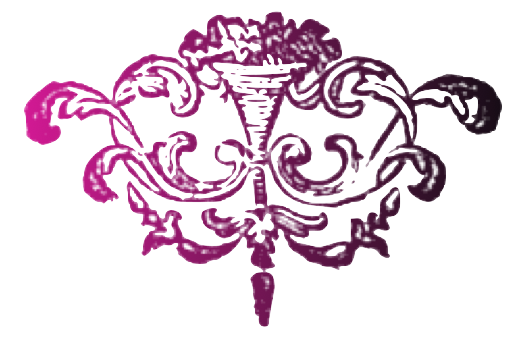
\includegraphics[width=.25\textwidth]{flourish2.png}
\end{center}
\vfill




\newpage

\section*{2$^{\textrm{\sffamily{e}}}$ Entr\'{e}e \\ Les Incas du P\'{e}rou (The Incas of Peru)}\secheadr{Act 2}
\addcontentsline{toc}{section}{2. Les Incas du P\'{e}rou}
\addtoendnotes{\protect\subsection*{Act 2}}
\addtoendnotes{\protect\addcontentsline{toc}{subsection}{Act 2}}

\begin{pairs}
\begin{Leftside}
	\setline{1}
	\stanza
		\scene{Le th\'{e}\^{a}tre repr\'{e}sente un d\'{e}sert du P\'{e}rou, termin\'{e} par une montagne aride. Le sommet en est couronn\'{e} par la bouche d'un volcan form\'{e}e de rochers calcin\'{e}s et couverts de cendres.}
	\& 
	\endnumbering
\end{Leftside}
\begin{Rightside}
	\setline{1}
	\stanza
		\scene{The stage depicts a desert in Peru, ending in an arid mountain. The summit is crowned by the mouth of a volcano made of charred rocks and covered in ash.}
	\&
	\endnumbering
\end{Rightside} 
\Columns 
\end{pairs}

\subsection*{Sc\`{e}ne 1}
\addcontentsline{toc}{subsection}{Sc\`{e}ne 1}

\begin{pairs}
\begin{Leftside}
	\setline{2}
	\stanza
		\scene{Phani, Carlos, Officier espagnol.}
    \& 
    \endnumbering
\end{Leftside}
\begin{Rightside}
	\setline{2}
	\stanza
		\scene{Phani; Carlos, a Spanish officer.}
    \& 
    \endnumbering
\end{Rightside} 
\Columns 
\end{pairs}

\dialogue{Carlos}
\begin{pairs}
\begin{Leftside}
	\setline{3}
	\stanza
		Vous devez bannir de votre \^{a}me&
		La criminelle erreur qui s\'{e}duit les Incas.&
		Vous l'avez promis \`{a} ma flamme.&
		Pourquoi diff\'{e}rez-vous? Non, vous ne m'aimez pas\ldots{}
    \& 
    \endnumbering
\end{Leftside}
\begin{Rightside}
	\setline{3}
	\stanza
		You must banish from your soul&
		The criminal error that seduces the Incas.&
		You have promised it to my flame.&
		Why do you defer? No, you do not love me\ldots{}
    \& 
    \endnumbering
\end{Rightside} 
\Columns 
\end{pairs}

\dialogue{Phani}
\begin{pairs}
\begin{Leftside}
	\setline{7}
	\stanza
		Que vous p\'{e}n\'{e}trez mal mon secret embarras! &
		Quel injuste soup\c{c}on! \ldots{}Quoi! Sans inqui\'{e}tude,&
		Brise-t-on \`{a} la fois&
		Les liens du sang et des lois?&
		Excusez mon incertitude!
    \& 
    \endnumbering
\end{Leftside}
\begin{Rightside}
	\setline{7}
	\stanza
		How poorly you comprehend my secret shame! &
		What unjust suspicion! \ldots{}What, without concern,&
		Do we loosen at one time &
		Both ties of blood and of laws? &
		Excuse my uncertainty!
    \& 
    \endnumbering
\end{Rightside} 
\Columns 
\end{pairs}

\dialogue{Carlos}
\begin{pairs}
\begin{Leftside}
	\setline{12}
	\stanza
		Dans un culte fatal, qui peut vous arr\^{e}ter?
    \& 
    \endnumbering
\end{Leftside}
\begin{Rightside}
	\setline{12}
	\stanza
		In a fatal cult, who can stop you?
    \& 
    \endnumbering
\end{Rightside} 
\Columns 
\end{pairs}

\dialogue{Phani}
\begin{pairs}
\begin{Leftside}
	\setline{13}
	\stanza
		Ne croyez point, Carlos, que ma raison balance!&
		Mais de nos fiers Incas je crains la violence\ldots{}
    \& 
    \endnumbering
\end{Leftside}
\begin{Rightside}
	\setline{13}
	\stanza
		Do not believe, Carlos, that my judgment wavers!&
		But I fear violence from our proud Incas\ldots{}
    \& 
    \endnumbering
\end{Rightside} 
\Columns 
\end{pairs}

\dialogue{Carlos}
\begin{pairs}
\begin{Leftside}
	\setline{15}
	\stanza
		Ah! Pouvez-vous les redouter?
    \& 
    \endnumbering
\end{Leftside}
\begin{Rightside}
	\setline{15}
	\stanza
		Ah! Can you fear them?
    \& 
    \endnumbering
\end{Rightside} 
\Columns 
\end{pairs}

\dialogue{Phani}
\begin{pairs}
\begin{Leftside}
	\setline{16}
	\stanza
		Sur ces monts, leurs derniers asiles,&
		La f\^{e}te du Soleil va les ressembler tous\ldots{}
    \& 
    \endnumbering
\end{Leftside}
\begin{Rightside}
	\setline{16}
	\stanza
		On these mountains, their final asylums,&
		They will all look alike during the Feast of the Sun\ldots{}
    \& 
    \endnumbering
\end{Rightside} 
\Columns 
\end{pairs}
 
\dialogue{Carlos}
\begin{pairs}
\begin{Leftside}
	\setline{18}
	\stanza
		Du trouble de leurs jeux, que ne profitons-nous?
    \& 
    \endnumbering
\end{Leftside}
\begin{Rightside}
	\setline{18}
	\stanza
		Why don't we take advantage of the disorder from their games?
    \& 
    \endnumbering
\end{Rightside} 
\Columns 
\end{pairs}

\dialogue{Phani}
\begin{pairs}
\begin{Leftside}
	\setline{19}
	\stanza
		Ils observent mes pas\ldots{}
    \& 
    \endnumbering
\end{Leftside}
\begin{Rightside}
	\setline{19}
	\stanza
		They watch my every step\ldots{}
    \& 
    \endnumbering
\end{Rightside} 
\Columns 
\end{pairs}

\dialogue{Carlos}
\begin{pairs}
\begin{Leftside}
	\setline{20}
	\stanza
		Leurs soins sont inutiles,&
		Si vous m'acceptez pour \'{e}poux.
    \& 
    \endnumbering
\end{Leftside}
\begin{Rightside}
	\setline{20}
	\stanza
		Their cares are pointless&
		If you accept me as husband.
    \& 
    \endnumbering
\end{Rightside} 
\Columns 
\end{pairs}

\dialogue{Phani}
\begin{pairs}
\begin{Leftside}
	\setline{22}
	\stanza
		Carlos, allez, pressez ce moment favorable,&
		D\'{e}livrez-moi d'un s\'{e}jour d\'{e}testable!&
		Mais ne venez pas seul ... Quel funeste malheur!&
		Si votre mort ... Le peuple est barbare, implacable,&
		Et quelquefois le nombre accable&
		La plus intr\'{e}pide valeur;&
		Ciel!
    \& 
    \endnumbering
\end{Leftside}
\begin{Rightside}
	\setline{22}
	\stanza
		Carlos, go, use this opportunity,&
		Deliver me from a detestable stay!&
		But do not come alone\ldots{} That would be deadly!&
		If your death\ldots{} The people are barbaric, cruel,&
		And sometimes a great number can overwhelm&
		The most fearless valor;&
		Heaven!
    \& 
    \endnumbering
\end{Rightside} 
\Columns 
\end{pairs}

\dialogue{Carlos}
\begin{pairs}
\begin{Leftside}
	\setline{29}
	\stanza
		Pouviez-vous \^{e}tre alarm\'{e}e?&
		Oubliez-vous que dans ces lieux&
		Un seul de nos guerriers triomphe d'une arm\'{e}e?
    \& 
    \endnumbering
\end{Leftside}
\begin{Rightside}
	\setline{29}
	\stanza
		Could you be alarmed?&
		Did you forget that in these places&
		A single one of our warriors is triumphant over an army?
    \& 
    \endnumbering
\end{Rightside} 
\Columns 
\end{pairs}

\dialogue{Phani}
\begin{pairs}
\begin{Leftside}
	\setline{32}
	\stanza
		Je sais vos exploits glorieux,&
		Et qu'\`{a} votre courage il n'est rien d'impossible.&
		Cependant, cher Carlos, empruntez du secours!
    \& 
    \endnumbering
\end{Leftside}
\begin{Rightside}
	\setline{32}
	\stanza
		I know your glorious exploits&
		And that to your courage everything is possible.&
		However, dear Carlos, rely on support!
    \& 
    \endnumbering
\end{Rightside} 
\Columns 
\end{pairs}

\dialogue{Carlos}
\begin{pairs}
\begin{Leftside}
	\setline{35}
	\stanza
		Que craignez-vous?
    \& 
    \endnumbering
\end{Leftside}
\begin{Rightside}
	\setline{35}
	\stanza
		What do you fear?
    \& 
    \endnumbering
\end{Rightside} 
\Columns 
\end{pairs}

\dialogue{Phani}
\begin{pairs}
\begin{Leftside}
	\setline{36}
	\stanza
		H\'{e}las! Je suis sensible;&
		Lorsque l'on aime, on craint toujours.
    \& 
    \endnumbering
\end{Leftside}
\begin{Rightside}
	\setline{36}
	\stanza
		Alas, I am sensitive!&
		If one loves, one fears everything.
    \& 
    \endnumbering
\end{Rightside} 
\Columns 
\end{pairs}

\subsection*{Sc\`{e}ne 2}
\addcontentsline{toc}{subsection}{Sc\`{e}ne 2}

\begin{pairs}
\begin{Leftside}
	\setline{38}
	\stanza
		\scene{Phani seule}
    \& 
    \endnumbering
\end{Leftside}
\begin{Rightside}
	\setline{38}
	\stanza
		\scene{Phani alone}
    \& 
    \endnumbering
\end{Rightside} 
\Columns 
\end{pairs}

\dialogue{Phani}
\begin{pairs}
\begin{Leftside}
	\setline{39}
	\stanza
		Viens, Hymen, viens m'unir au vainqueur que j'adore!&
		Forme tes noeuds, encha\^{i}ne-moi!&
		Dans ces tendres instants o\`{u} ma flamme t'implore,&
		L'amour m\^{e}me n'est pas plus aimable que toi.
    \& 
    \endnumbering
\end{Leftside}
\begin{Rightside}
	\setline{39}
	\stanza
		Hymen, come join me to the conqueror whom I love!&
		Tie your knots, enchain me!&
		In the tender moments where my passion implores you,&
		Even love itself is less lovely than you.
    \& 
    \endnumbering
\end{Rightside} 
\Columns 
\end{pairs}	

\subsection*{Sc\`{e}ne 3}
\addcontentsline{toc}{subsection}{Sc\`{e}ne 3}

\begin{pairs}
\begin{Leftside}
	\setline{43}
	\stanza
		\scene{Phani, Huascar}
    \& 
    \endnumbering
\end{Leftside}
\begin{Rightside}
	\setline{43}
	\stanza
		\scene{Phani, Huascar}
    \& 
    \endnumbering
\end{Rightside} 
\Columns 
\end{pairs}

\dialogue{Huascar}
\begin{pairs}
\begin{Leftside}
	\setline{44}
	\stanza
		\stage{\`{a} part}&
		Elle est seule\ldots{} parlons! L'instant est favorable\ldots{}&
		Mais je crains d'un rival l'obstacle redoutable.&
		Parlons au nom des Dieux pour surprendre son coeur!&
		Tout ce que dit l'Amour est toujours pardonnable,&
		Et le ciel que je sers doit servir mon ardeur.
	\&
	\stanza		
		\setline{50}\stage{\`{a} Phani}&
		Le dieu de nos climats dans ce beau jour m'inspire.&
		Princesse, le soleil daigne veiller sur vous,&
		Et lui-m\^{e}me dans notre empire,&
		Il pr\'{e}tend par ma voix vous nommer un \'{e}poux.&
		Vous fr\'{e}missez\ldots{} D'o\`{u} vient que votre coeur soupire?
	\&
	\stanza
		\setline{56}Ob\'{e}issons sans balancer&
		Lorsque le ciel commande!&
		Nous ne pouvons trop nous presser&
		D'accorder ce qu'il nous demande;&
		Y r\'{e}fl\'{e}chir, c'est l'offenser.
    \& 
    \endnumbering
\end{Leftside}
\begin{Rightside}
	\setline{44}
	\stanza
		\stage{aside}&
		She is alone\ldots{} let us speak! The moment is favorable\ldots{}&
		But I fear the formidable obstacle of a rival.&
		We'll implore the gods to surprise her heart!&
		Everything said to Cupid is always pardonable,&
		And the heaven that I serve must serve my ardor.
	\&
	\stanza
		\setline{50}\stage{to Phani}&
		The god of our climes in this beautiful day inspires me.&
		Princess, the sun himself deigns to watch out for you,&
		And he himself in our empire,&
		He argues through my voice for you to name a husband.&
		You shudder\ldots{} Why does your heart sigh?
	\&
	\stanza
		\setline{56}Obey without hesitation&
		When the sky commands it!&
		No rushing is too much&
		For us to grant what is demanded of us;&
		To first think about it, that's the offense.
    \&
    \endnumbering
\end{Rightside} 
\Columns 
\end{pairs}

\dialogue{Phani}
\begin{pairs}
\begin{Leftside}
	\setline{61}
	\stanza
		Non, non, je ne crois pas tout ce que l'on assure &
		En attestant les cieux;&
		C'est souvent l'imposture &
		Qui parle au nom des Dieux.
    \& 
    \endnumbering
\end{Leftside}
\begin{Rightside}
	\setline{61}
	\stanza
		No, no, I do not believe all that we hear &
		As attesting the heavens; &
		It is often the imposter &
		Who speaks in the name of the Gods.
    \& 
    \endnumbering
\end{Rightside} 
\Columns 
\end{pairs}

\dialogue{Huascar}
\begin{pairs}
\begin{Leftside}
	\setline{65}
	\stanza
		Pour les Dieux et pour moi, quelle coupable injure! &
		Je sais ce qui produit votre incr\'{e}dulit\'{e}, &
		C'est l'amour! Dans votre \^{a}me, il est seul \'{e}cout\'{e}!
    \& 
    \endnumbering
\end{Leftside}
\begin{Rightside}
	\setline{65}
	\stanza
		For the Gods and for me, what culpable abuse!&
		I know that which creates your incredulity---&
		It's love! In your soul, love alone is heard!
    \& 
    \endnumbering
\end{Rightside} 
\Columns 
\end{pairs}

\dialogue{Phani}
\begin{pairs}
\begin{Leftside}
	\setline{68}
	\stanza
		L'amour! Que croyez-vous?
    \& 
    \endnumbering
\end{Leftside}
\begin{Rightside}
	\setline{68}
	\stanza
		Love! What do you believe?
    \& 
    \endnumbering
\end{Rightside} 
\Columns 
\end{pairs}

\dialogue{Huascar}
\begin{pairs}
\begin{Leftside}
	\setline{69}
	\stanza
		Oui, vous aimez, perfide,&
		Un de nos vainqueurs inhumains.&
		Ciel! Mettras-tu toujours tes armes dans leurs mains?
    \& 
    \endnumbering
\end{Leftside}
\begin{Rightside}
	\setline{69}
	\stanza
		Yes, traitor, you love&
		One of our inhumane conquerors.&
		Heaven! Will you always put your weapons in their hands?
    \& 
    \endnumbering
\end{Rightside} 
\Columns 
\end{pairs}

\dialogue{Phani}
\begin{pairs}
\begin{Leftside}
	\setline{72}
	\stanza
		Redoutez le Dieu qui les guide!
    \& 
    \endnumbering
\end{Leftside}
\begin{Rightside}
	\setline{72}
	\stanza
		Fear the God who guides them!
    \& 
    \endnumbering
\end{Rightside} 
\Columns 
\end{pairs}

\dialogue{Huascar}
\begin{pairs}
\begin{Leftside}
	\setline{73}
	\stanza
		C'est l'or qu'avec empressement,&
		Sans jamais s'assouvir, ces barbares d\'{e}vorent.&
		L'or qui de nos autels ne fait que l'ornement&
		Est le seul Dieu que nos tyrans adorent.
    \& 
    \endnumbering
\end{Leftside}
\begin{Rightside}
	\setline{73}
	\stanza
		It is gold that, with eagerness,&
		Without satiety, these barbarians devour.&
		The gold which on our altars is only ornament&
		Is the sole god our tyrants adore.
    \& 
    \endnumbering
\end{Rightside} 
\Columns 
\end{pairs}

\dialogue{Phani}
\begin{pairs}
\begin{Leftside}
	\setline{77}
	\stanza
		T\'{e}m\'{e}raire! Que dites-vous!&
		R\'{e}v\'{e}rez leur puissance, et craignez leur courroux.&
		Pour leur obtenir vos hommages,&
		Faut-il des miracles nouveaux?&
		Vous avez vu, de nos rivages,&
		Leurs villes voler sur les eaux;&
		Vous avez vu, dans l'horreur de la guerre,&
		Leur invincible bras disposer du tonnerre\ldots{}
    \& 
    \endnumbering
\end{Leftside}
\begin{Rightside}
	\setline{77}
	\stanza
		Such foolhardy words!&
		Revere their power, and fear their wrath.&
		In order to get your tributes,&
		Must there be new miracles?&
		From our shores, you have seen&
		Their cities flying over the waters;&
		In the horror of war, you have seen&
		Their invincible arms creating thunder\ldots{}
    \& 
    \endnumbering
\end{Rightside} 
\Columns 
\end{pairs}

\subsection*{Sc\`{e}ne 4}
\addcontentsline{toc}{subsection}{Sc\`{e}ne 4}

\begin{pairs}
\begin{Leftside}
	\setline{85}
	\stanza
		\scene{Huascar et un Inca, son confident. On entend un pr\'{e}lude qui annonce la f\^{e}te du Soleil.}
    \& 
    \endnumbering
\end{Leftside}
\begin{Rightside}
	\setline{85}
	\stanza
		\scene{Huascar and an Inca, his confidant. We hear a prelude announcing the Feast of the Sun.}
    \& 
    \endnumbering
\end{Rightside} 
\Columns 
\end{pairs}

\dialogue{Huascar}
\begin{pairs}
\begin{Leftside}
	\setline{86}
	\stanza
		\stage{\`{a} part}&
		On vient, dissimulons mes transports \`{a} leurs yeux!
	\&
	\stanza
		\setline{88}\stage{\`{a} l'Inca qu'il appelle}&
		Vous savez mon projet. Allez, qu'on m'ob\'{e}isse\ldots{}
	\&
	\stanza
		\setline{90}\stage{\`{a} part}&
		Je n'ai donc plus pour moi qu'un barbare artifice,&
		Qui de flamme et de sang inondera ces lieux.&
		Mais que ne risque point un amour furieux?
    \& 
    \endnumbering
\end{Leftside}
\begin{Rightside}
	\setline{86}
	\stanza
		\stage{aside}&
		Someone comes\ldots{} let us conceal my tricks from their eyes!
	\&
	\stanza
		\setline{88}\stage{calling to the Inca}&
		You know my project. Go ahead, so that she obeys me\ldots{}
	\&
	\stanza
		\setline{90}\stage{aside}&
		I don't have much more for me than a barbaric trick,&
		Which will flood this place with flame and blood.&
		But what wouldn't an angry love risk?
    \& 
    \endnumbering
\end{Rightside} 
\Columns 
\end{pairs}

\subsection*{Sc\`{e}ne 5}
\addcontentsline{toc}{subsection}{Sc\`{e}ne 5}

\begin{pairs}
\begin{Leftside}
	\setline{94}
	\stanza
		\scene{F\^{e}te du Soleil}&
		\scene{Huascar, Phani, ramen\'{e}e par des Incas, Pallas et Incas, Sacrificateurs, P\'{e}ruviens et P\'{e}ruviennes}
    \& 
    \endnumbering
\end{Leftside}
\begin{Rightside}
	\setline{94}
	\stanza
		\scene{Feast of the Sun}&
		\scene{Huascar, Phani, brought by the Incas, Pallas and Incas, Priests, Peruvian men and women}
    \& 
    \endnumbering
\end{Rightside} 
\Columns 
\end{pairs}

\dialogue{Huascar}
\begin{pairs}
\begin{Leftside}
	\setline{96}
	\stanza
		Soleil, on a d\'{e}truit tes superbes asiles,&
		Il ne te reste plus de temple que nos coeurs.&
		Daigne nous \'{e}couter dans ces d\'{e}serts tranquilles!&
		Le z\`{e}le est pour les Dieux le plus cher des honneurs.
    \& 
    \endnumbering
\end{Leftside}
\begin{Rightside}
	\setline{96}
	\stanza
		Sun, we destroyed your superb havens,&
		Leaving no temple for you but our hearts.&
		Deign to hear us, in these tranquil deserts!&
		Zeal is, for the gods, the highest of honors.
   	\&
    \endnumbering
\end{Rightside} 
\Columns 
\end{pairs}

\balletnum{preludeadoration}{Pr\'{e}lude pour l'adoration du Soleil}{Prelude for the adoration of the Sun}

\begin{pairs}
\begin{Leftside}
	\setline{100}
	\stanza
		\stage{Les Pallas et Incas font leur adoration au Soleil}
    \& 
    \endnumbering
\end{Leftside}
\begin{Rightside}
	\setline{100}
	\stanza
		\stage{The Pallas and Incas display their adoration to the Sun}
    \& 
    \endnumbering
\end{Rightside} 
\Columns 
\end{pairs}

\dialogue{Huascar}
\begin{pairs}
\begin{Leftside}
	\setline{101}
	\stanza
		Brillant soleil, jamais nos yeux, dans ta carri\`{e}re,&
		N'ont vu tomber de noirs frimas,&
		Et tu r\'{e}pands dans nos climats&
		Ta plus \'{e}clatante lumi\`{e}re.
    \& 
    \endnumbering
\end{Leftside}
\begin{Rightside}
	\setline{101}
	\stanza
		Brilliant sun, in your career, our eyes &
		Have never seen black frost falling,&
		And you spread throughout our climes&
		Your brightest light.
    \& 
    \endnumbering
\end{Rightside} 
\Columns 
\end{pairs}

\balletnum{airdesincas}{Air des Incas pour la d\'{e}votion du Soleil}{Air of the Incas for the Sun's devotion}

\song{Danse de P\'{e}ruviens et de P\'{e}ruviennes}

\dialogue{Huascar}
\begin{pairs}
\begin{Leftside}
	\setline{105}
	\stanza
		Clair flambeau du monde,&
		L'air, la terre et l'onde&
		Ressentent tes bienfaits!&
		Clair flambeau du monde,&
		L'air, la terre et l'onde&
		Te doivent leurs attraits!
    \& 
    \endnumbering
\end{Leftside}
\begin{Rightside}
	\setline{105}
	\stanza
		Clear torch of the world,&
		The air, the earth, and the wave&
		All feel your kindness!&
		Clear torch of the world,&
		The air, the earth, and the wave&
		All owe you their charms!
    \& 
    \endnumbering
\end{Rightside} 
\Columns 
\end{pairs}

\dialogue{Choeur}
\begin{pairs}
\begin{Leftside}
	\setline{111}
	\stanza
		Clair flambeau du monde,&
		L'air, la terre et l'onde&
		Ressentent tes bienfaits!&
		Clair flambeau du monde,&
		L'air, la terre et l'onde&
		Te doivent leurs attraits!
    \& 
    \endnumbering
\end{Leftside}
\begin{Rightside}
	\setline{111}
	\stanza
		Clear torch of the world,&
		The air, the earth, and the wave&
		All feel your kindness!&
		Clear torch of the world,&
		The air, the earth, and the wave&
		All owe you their charms!
    \& 
    \endnumbering
\end{Rightside} 
\Columns 
\end{pairs}

\dialogue{Huascar}
\begin{pairs}
\begin{Leftside}
	\setline{117}
	\stanza
		Par toi dans nos champs tout abonde.&
		Nous ne pouvons compter les biens que tu nous fais.&
		Chantons-les seulement! Que l'\'{e}cho nous r\'{e}ponde!&
		Que ton nom dans nos bois retentisse \`{a} jamais!&
		Tu laisses l'univers dans une nuit profonde,&
		Lorsque tu disparais;&
		Et nos yeux, en perdant ta lumi\`{e}re f\'{e}conde,&
		Perdent tous leurs plaisirs; la beaut\'{e} perd ses traits.
    \& 
    \endnumbering
\end{Leftside}
\begin{Rightside}
	\setline{117}
	\stanza
		Through you, all abounds in our fields.&
		We cannot count your blessings.&
		Let us sing only of them! Let the echo meet us!&
		May your name forever resound in our woods!&
		You leave the universe in profound darkness&
		When you disappear;&
		And our eyes, in losing your fecund light,&
		Lose all their pleasures; beauty loses its features.
    \& 
    \endnumbering
\end{Rightside} 
\Columns 
\end{pairs}

\song{Loure en rondeau}

\dialogue{Huascar}
\begin{pairs}
\begin{Leftside}
	\setline{125}
	\stanza
		Permettez, astre du jour,&
		Qu'en chantant vos feux nous chantions d'autres flammes;&
		Partagez, astre du jour,&
		L'encens de nos \^{a}mes&
		Avec le tendre amour.&
		Le soleil, en guidant nos pas,&
		R\'{e}pand ses app\^{a}ts&
		Dans les routes qu'il pare.&
		Raison, quand malgr\'{e} tes soins,&
		L'amour nous \'{e}gare,&
		Nous pla\^{i}t-il moins?&
		Vous brillez, astre du jour,&
		Vous charmez nos yeux par l'\'{e}clat de vos flammes!&
		Vous brillez, astre du jour! L'astre de nos \^{a}mes,&
		C'est le tendre amour.&
		De nos bois chassez la tristesse,&
		R\'{e}gnez-y sans cesse, Dieux de nos coeurs!&
		De la nuit le coile sombre&
		Sur vos attraits n'\'{e}tend jamais son ombre;&
 		Tous les temps, aimables vainqueurs,&
 		Sont marqu\'{e}s par vos faveurs.
    \& 
	\stanza
		\stage{On danse, et la f\^{e}te est troubl\'{e}e par un tremblement de terre.}
	\&
    \endnumbering
\end{Leftside}
\begin{Rightside}
	\setline{125}
	\stanza
		Daystar, permit,&
		In singing of your fires, that which we sang of other flames;&
		Share, Daystar,&
		The incense of our souls&
		With tender love.&
		The sun, guiding our steps,&
		Spreads his baits&
		In the routes that he adorns.&
		Therefore, when in spite of your care,&
		Love leads us astray,&
		Does it please us less?&
		Shine, Daystar!&
		Charm our eyes by the brightness of your flames!&
		Shine, Daystar! The star of our souls,&
		It is the tenderest love.&
		Chase sadness from our woods,&
		And reign there forever, God of our hearts!&
		Though the gloomy night coils&
		Around your charms, it cannot extend its shadow;&
 		All the time, kind victors,&
 		Are marked by your favors.
    \& 
	\stanza
		\stage{They dance, and the feast is troubled by an earthquake.}
	\&
    \endnumbering
\end{Rightside} 
\Columns 
\end{pairs}

\song{1$^{\textrm{er}}$  Gavotte}

\song{2$^{\textrm{e}}$ Gavotte en Rondeau}

\begin{pairs}
\begin{Leftside}
	\setline{148}
	\stanza
		\stage{Tremblement de terre}
    \& 
    \endnumbering
\end{Leftside}
\begin{Rightside}
	\setline{148}
	\stanza
		\stage{Earthquake}
    \& 
    \endnumbering
\end{Rightside} 
\Columns 
\end{pairs}

\dialogue{Choeur}
\begin{pairs}
\begin{Leftside}
	\setline{149}
	\stanza
		Dans les ab\^{i}mes de la terre,&
		Les vents se d\'{e}clarent la guerre.
    \& 
	\stanza\skipnumbering
		\stage{L'air s'obscurcit, le tremblement redouble, le volcan s'allume et jette par tourbillons du feu et de la fum\'{e}e.}
	\&
	\stanza
		Les rochers embras\'{e}s s'\'{e}lancent dans les airs,&
		Et portent jusqu'aux cieux les flammes des enfers.
	\&
	\stanza
		\stage{L'\'{e}pouvante saisit les P\'{e}ruviens, l'assembl\'{e}e se disperse. Huascar arr\^{e}te Phani. Le tremblement de terre semble s'apaiser.}
	\&
    \endnumbering
\end{Leftside}
\begin{Rightside}
	\setline{149}
	\stanza
		In the depths of the earth,&
		Winds declare war.
	\& 
	\stanza\skipnumbering
		\stage{The air darkens, the trembling redoubles, and the volcano illuminates and erupts clouds of fire and smoke.}
	\&
	\stanza
		The fiery rocks dart into the air&
		And carry to heaven the flames of hell.
	\&
	\stanza
		\stage{Horror seizes the Peruvians, and the assembly scatters. Huascar stops Phani. The earthquake seems to subside.}
	\&
    \endnumbering
\end{Rightside} 
\Columns 
\end{pairs}

\subsection*{Sc\`{e}ne 6}
\addcontentsline{toc}{subsection}{Sc\`{e}ne 6}

\begin{pairs}
\begin{Leftside}
	\setline{155}
	\stanza
		\scene{Huascar, Phani}
    \& 
    \endnumbering
\end{Leftside}
\begin{Rightside}
	\setline{155}
	\stanza
		\scene{Huascar, Phani}
    \& 
    \endnumbering
\end{Rightside} 
\Columns 
\end{pairs}

\dialogue{Huascar}
\begin{pairs}
\begin{Leftside}
	\setline{156}
	\stanza
		\stage{\`{a} Phani qui traverse le th\'{e}\^{a}tre en s'enfuyant}&
		Arr\^{e}tez! Par ces feux le ciel vient de m'apprendre&
		Qu'\`{a} son arr\^{e}t il faut vous rendre,&
		Et l'hymen\ldots{}
    \& 
    \endnumbering
\end{Leftside}
\begin{Rightside}
	\setline{156}
	\stanza
		\stage{to Phani, fleeing across the stage}&
		Stop! By these lights the sky has just taught me&
		That it is necessary for you to follow by its judgment,&
		And marriage\ldots{}
    \& 
    \endnumbering
\end{Rightside} 
\Columns 
\end{pairs}

\dialogue{Phani}
\begin{pairs}
\begin{Leftside}
	\setline{160}
	\stanza
		Qu'allez-vous encore me r\'{e}v\'{e}ler?&
		O jour funeste! Dois-je croire&
		Que le ciel, jaloux de sa gloire,&
		Ne s'explique aux humains qu'en les faisant trembler?
    \& 
    \endnumbering
\end{Leftside}
\begin{Rightside}
	\setline{160}
	\stanza
		What more are you going to show me?&
		Oh, fatal day! Must I believe&
		That the sky, jealous of his glory,&
		Can explain himself to humans only by making them tremble?
    \& 
    \endnumbering
\end{Rightside} 
\Columns 
\end{pairs}

\dialogue{Huascar}
\begin{pairs}
\begin{Leftside}
	\setline{164}
	\stanza
		\stage{l'arr\^{e}tant encore}&
		Vous fuyez, quand les Dieux daignent vous appeler!&
		Eh bien! cruelle, eh bien! vous allez me conna\^{i}tre.&
		Suivez l'amour jaloux!
    \& 
    \endnumbering
\end{Leftside}
\begin{Rightside}
	\setline{164}
	\stanza
		\stage{stopping her again}&
		You flee when the gods deign to call you!&
		Well then, cruelly will you know me!&
		Follow jealous love!
    \& 
    \endnumbering
\end{Rightside} 
\Columns 
\end{pairs}

\dialogue{Phani}
\begin{pairs}
\begin{Leftside}
	\setline{168}
	\stanza
		\stage{se reculant}&
		Ton crime ose para\^{i}tre!
    \& 
    \endnumbering
\end{Leftside}
\begin{Rightside}
	\setline{168}
	\stanza
		\stage{recoiling}&
		Your crime dares to appear!
    \& 
    \endnumbering
\end{Rightside} 
\Columns 
\end{pairs}

\dialogue{Huascar}
\begin{pairs}
\begin{Leftside}
	\setline{170}
	\stanza
		Que l'on est criminel lorsque l'on ne pla\^{i}t pas!&
		Du moins en me suivant \'{e}vitez le tr\'{e}pas!\ldots{}
	\&
	\stanza\skipnumbering
		Ici je vois partout l'affreuse mort suivie&
		D'un redoutable embrasement.&
		Chaque instant peut de votre vie&
		Devenir le dernier moment.
    \& 
    \endnumbering
\end{Leftside}
\begin{Rightside}
	\setline{170}
	\stanza
		Oh, how one is criminal when one doesn't please!&
		At least in following me you avoid demise!\ldots{}
	\&
	\stanza\skipnumbering
		Here I see everywhere horrible death which follows&
		From a dreadful conflagration.&
		Each instant can become&
		The final moment of your life.
    \& 
    \endnumbering
\end{Rightside} 
\Columns 
\end{pairs}

\subsection*{Sc\`{e}ne 7}
\addcontentsline{toc}{subsection}{Sc\`{e}ne 7}

\begin{pairs}
\begin{Leftside}
	\setline{177}
	\stanza
		\scene{Phani, Huascar, Carlos}
    \& 
    \endnumbering
\end{Leftside}
\begin{Rightside}
	\setline{177}
	\stanza
		\scene{Phani, Huascar, Carlos}
    \& 
    \endnumbering
\end{Rightside} 
\Columns 
\end{pairs}

\dialogue{Huascar}
\begin{pairs}
\begin{Leftside}
	\setline{178}
	\stanza
		\stage{\`{a} Phani}&
		Quoi! Plus que le p\'{e}ril mon amour vous \'{e}tonne?&
		C'est trop me r\'{e}sister\ldots{}
    \& 
    \endnumbering
\end{Leftside}
\begin{Rightside}
	\setline{178}
	\stanza
		\stage{to Phani}&
		What! More than danger, my love surprises you?&
		It's too much to resist me\ldots{}
    \& 
    \endnumbering
\end{Rightside} 
\Columns 
\end{pairs}

\dialogue{Phani}
\begin{pairs}
\begin{Leftside}
	\setline{181}
	\stanza
		O ciel, entends mes voeux!
    \& 
    \endnumbering
\end{Leftside}
\begin{Rightside}
	\setline{181}
	\stanza
		Oh heaven, hear my wishes!
    \& 
    \endnumbering
\end{Rightside} 
\Columns 
\end{pairs}

\dialogue{Huascar}
\begin{pairs}
\begin{Leftside}
	\setline{182}
	\stanza
		C'est aux miens qu'il vous abandonne.
    \& 
    \endnumbering
\end{Leftside}
\begin{Rightside}
	\setline{182}
	\stanza
		Mine are that it abandons you.
    \& 
    \endnumbering
\end{Rightside} 
\Columns 
\end{pairs}

\dialogue{Carlos}
\begin{pairs}
\begin{Leftside}
	\setline{183}
	\stanza
		\stage{arrivant sur Huascar un poignard \`{a} la main}&
		Tu t'abuses, barbare!
    \& 
    \endnumbering
\end{Leftside}
\begin{Rightside}
	\setline{183}
	\stanza
		\stage{arriving at Huascar with a daggar in hand}&
		You are mistaken, barbarian!
    \& 
    \endnumbering
\end{Rightside} 
\Columns 
\end{pairs}

\dialogue{Phani}
\begin{pairs}
\begin{Leftside}
	\setline{185}
	\stanza
		Ah! Carlos! Je frissonne.&
		Le soleil jusqu'au fond des antres les plus creux&
		Vient d'allumer la terre, et son courroux pr\'{e}sage\ldots{}
    \& 
    \endnumbering
\end{Leftside}
\begin{Rightside}
	\setline{185}
	\stanza
		Ah, Carlos! I shudder.&
		To the bottoms of the deepest caverns, the Sun&
		Just lit up the earth, and his wrath forebodes\ldots{}
    \& 
    \endnumbering
\end{Rightside} 
\Columns 
\end{pairs}

\dialogue{Carlos}
\begin{pairs}
\begin{Leftside}
	\setline{188}
	\stanza
		Princesse, quelle erreur!&
		C'est le ciel qu'elle outrage.&
		Cet embrasement dangereux&
		Du soleil n'est point l'ouvrage,&
		Il est celui de sa rage.&
		Un seul rocher jet\'{e} dans ces gouffres affreux,&
		Y r\'{e}veillant l'ardeur de ces terribles feux,&
		Suffit pour exciter un si fatal ravage.&
		Le perfide esp\'{e}rait vous tromper dans ce jour,&
		Et que votre terreur servirait son amour.&
		Sur ces monts mes guerriers punissent ses complices,&
		Ils vont trouver dans ces noirs pr\'{e}cipices&
		Des tombeaux dignes d'eux.
	\&
	\stanza\skipnumbering
		\stage{\`{a} Huascar}&
		Mais il te faut de plus cruels supplices.
	\&
	\stanza
		\stage{\`{a} Phani}&
		Accordez votre main \`{a} son rival heureux,&
		C'est l\`{a} son ch\^{a}timent!
    \& 
    \endnumbering
\end{Leftside}
\begin{Rightside}
	\setline{188}
	\stanza
		Princess, what a mistake!&
		It is the sky whom the earth insults.&
		This dangerous blaze&
		Is not the sun's work;&
		The sun is the object of her anger.&
		A single rock thrown into those dreadful chasms,&
		Awakens there the passion of these terrible fires,&
		Enough to excite such a fatal disaster.&
		The traitor hopes to mislead you this day,&
		And that your terror would serve his love.&
		On those mountains, my warriors punish his accomplices.&
		They will find, in dark ravines,&
		Tombs worthy of them.
	\&
	\stanza\skipnumbering
		\stage{to Huascar}&
		But you deserve crueler torture.
	\&
	\stanza
		\stage{to Phani}&
		Grant your hand to his fortunate rival:&
		That will be his punishment!
    \& 
    \endnumbering
\end{Rightside} 
\Columns 
\end{pairs}

\dialogue{Huascar}
\begin{pairs}
\begin{Leftside}
	\setline{206}
	\stanza
		Ciel! Qu'il est rigoureux
    \& 
    \endnumbering
\end{Leftside}
\begin{Rightside}
	\setline{206}
	\stanza
		Heaven! He is severe.
    \& 
    \endnumbering
\end{Rightside} 
\Columns 
\end{pairs}

\dialogue{Phani, Carlos}
\begin{pairs}
\begin{Leftside}
	\setline{207}
	\stanza
		Pour jamais, l'amour nous engage.&
		Non, non, rien n'est \'{e}gal \`{a} ma f\'{e}licit\'{e}.&
		Ah! Mon coeur a bien m\'{e}rit\'{e}&
		Le sort qu'avec vous il partage.
    \& 
    \endnumbering
\end{Leftside}
\begin{Rightside}
	\setline{207}
	\stanza
		Love engages us forever.&
		No, no, nothing compares to my bliss.&
		Ah! My heart has well earned&
		The fate that it shares with you.
    \& 
    \endnumbering
\end{Rightside} 
\Columns 
\end{pairs}

\dialogue{Huascar}
\begin{pairs}
\begin{Leftside}
	\setline{211}
	\stanza
		Non, non, rien n'\'{e}gale ma rage.&
		Je suis t\'{e}moin de leur f\'{e}licit\'{e}.&
		Faut-il que mon coeur irrit\'{e}&
		Ne puisse \^{e}tre veng\'{e} d'un si cruel outrage?
    \& 
    \endnumbering
\end{Leftside}
\begin{Rightside}
	\setline{211}
	\stanza
		No, no, nothing compares to my rage.&
		I am a witness of their bliss.&
		Must my irritated heart&
		Be beyond vengeance of so cruel an outrage?
    \& 
    \endnumbering
\end{Rightside} 
\Columns 
\end{pairs}

\subsection*{Sc\`{e}ne 8}
\addcontentsline{toc}{subsection}{Sc\`{e}ne 8}

\begin{pairs}
\begin{Leftside}
	\setline{215}
	\stanza
		\scene{Les m\^{e}mes. Le volcan se rallume, et le tremblement de terre recommence.}
    \& 
    \endnumbering
\end{Leftside}
\begin{Rightside}
	\setline{215}
	\stanza
		\scene{The same place. The volcano is once again active, and the earthquake resumes.}
    \& 
    \endnumbering
\end{Rightside} 
\Columns 
\end{pairs}

\dialogue{Huascar}
\begin{pairs}
\begin{Leftside}
	\setline{216}
	\stanza
		La flamme se rallume encore,&
		Loin de l'\'{e}viter, je l'implore\ldots{}&
		Ab\^{i}mes embras\'{e}s, j'ai trahi les autels.&
		Exercez l'emploi du tonnerre,&
		Vengez les droits des immortels,&
		D\'{e}chirez le sein de la terre&
		Sous mes pas chancelants!&
		Renversez, dispersez ces arides montagnes,&
		Lancez vos feux dans ces tristes campagnes,&
		Tombez sur moi, rochers br\^{u}lants.
    \& 
    \endnumbering
\end{Leftside}
\begin{Rightside}
	\setline{216}
	\stanza
		The flame returns again,&
		I beg for distance to avoid it\ldots{}&
		Blazing depths, I have betrayed the altars.&
		Exercise the use of the thunder,&
		Avenge the rights of the immortals,&
		Rip the breast of the earth&
		Beneath my unsteady footsteps!&
		Spill, scatter these arid mountains,&
		Launch your fires in this sad countryside,&
		Fall upon me, hot rocks.
    \& 
    \endnumbering
\end{Rightside} 
\Columns 
\end{pairs}

\begin{pairs}
\begin{Leftside}
	\setline{226}
	\stanza
		\stage{Le volcan vomit des rochers enflamm\'{e}s qui \'{e}crasent le criminel Huascar.}
    \& 
    \endnumbering
\end{Leftside}
\begin{Rightside}
	\setline{226}
	\stanza
		\stage{The volcano vomits fiery rocks that crush the criminal Huascar.}
    \& 
    \endnumbering
\end{Rightside} 
\Columns 
\end{pairs}

% \newpage
% 
% \section*{Act 3.~Les Fleurs (The Flowers)}
% \addcontentsline{toc}{section}{Act 3.~Les Fleurs}

\newpage

\section*{4$^{\textrm{\sffamily{e}}}$ Entr\'{e}e \\ Les sauvages (The Savages of America)}\secheadr{Act 4}
\addcontentsline{toc}{section}{4. Les sauvages}
\addtoendnotes{\protect\subsection*{Act 4}}
\addtoendnotes{\protect\addcontentsline{toc}{subsection}{Act 4}}
\addtoendnotes{\begingroup%
\parindent 4ex%
\parskip 0ex%
Fuzelier added the fourth act in 1736, seven months after the opera's premiere. The French noun \emph{sauvage}, found in the title and elsewhere in the act, has an obvious cognate in the English \emph{savage}, a word once often used to describe the native peoples of many lands encroached by colonial interests. The French adjective carries more nuance than it does today in English---suggesting ``unspoiled'' or ``uncorrupted,'' among other things. But the noun form also refers specifically to the native peoples of America, in the same way English until recently employed the word ``Indian'' to that same effect. The editors of a later edition of the opera's score clarifies this parallel evolution of the linguistic concept in French as it has in English: The 1761 sketch for a costume worn by the actress who plays Phani in the second act is described as that of ``une sauvagesse,'' clarifying further for the contemporary reader, ``ou Indienne de l'Am\'{e}rique''---`a [female] savage, or [female] Indian of America' \autocite[viii]{avant-propos:Rameau:1902aa}. A reproduction of this sketch is included on page~\pageref{phaniimage} at the end of the fourth act \autocite[from][lxiii]{commentaire-bibliographique:Rameau:1902aa}.

Apart from the title, where the context of these historical, linguistic resonances still ought to be felt, I've translated \emph{sauvage} primarily as ``native,'' except where the combination \emph{nation sauvage} would have rendered the awkward ``native nation.'' In these places, I have chosen the not-anachronistic alternative of ``Indian nation.'' \endgroup\newline}

\begin{pairs}
\begin{Leftside}
	\setline{1}
	\stanza
		\scene{Le th\'{e}\^{a}tre repr\'{e}sente un bosquet d'une for\^{e}t de l'Am\'{e}rique, voisine des colonies fran\c{c}aises et espagnoles o\`{u} doit se c\'{e}l\'{e}brer la c\'{e}r\'{e}monie du Grand Calumet de la Paix.}
	\& 
	\endnumbering
\end{Leftside}
\begin{Rightside}
	\setline{1}
	\stanza
		\scene{The stage depicts a forest grove in America, near the French and Spanish colonies, the place for conducting the ritual of the Great Pipe of Peace.}
	\&
	\endnumbering
\end{Rightside} 
\Columns 
\end{pairs}

\subsection*{Sc\`{e}ne 1}
\addcontentsline{toc}{subsection}{Sc\`{e}ne 1}

\begin{pairs}
\begin{Leftside}
	\setline{2}
	\stanza
		\scene{Adario commandant les guerriers de la nation sauvage.} &
		\scene{On entend les fanfares des trompettes fran\c{c}aises.}
    \& 
    \endnumbering
\end{Leftside}
\begin{Rightside}
	\setline{2}
	\stanza
		\scene{Adario commanding the warriors of the Indian nation.} &
		\scene{We hear the fanfares of French trumpets.}
    \& 
    \endnumbering
\end{Rightside} 
\Columns 
\end{pairs}

\begin{center}
	\textbf{\textsc{Adario}}
\end{center}
\begin{pairs}
\begin{Leftside}
	\setline{4}
	\stanza
		Nos guerriers, par mon ordre unis \`{a} nos vainqueurs,&
		Vont ici de la paix c\'{e}l\'{e}brer les douceurs; &
		Mon coeur seul dans ces lieux trouve encor des alarmes. &
		Je vois deux \'{e}trangers illustres par les armes, &
		\'{E}pris de l'objet de mes voeux; &
		Je crains leurs soupirs dangereux, &
		Et que leur sort brillant pour Zima n'ait des charmes. &
		Rivaux de mes exploits, rivaux de mes amours, &
		H\'{e}las! dois-je toujours & 
		Vous c\'{e}der la victoire? &
		Ne paraissez-vous dans nos bois &
		Que pour triompher \`{a} la fois &
		De ma tendresse et de ma gloire? &
		\stage{apercevant ses rivaux} &
		Ciel! Ils cherchent Zima\ldots{} voudrait-elle changer? &
		Cachons-nous\ldots{} apprenons ce que je dois en croire! &
		Sachons et si je dois et sur qui me venger! &
		\stage{Il se cache \`{a} l'entr\'{e}e de la for\^{e}t et les observe.}
    \& 
    \endnumbering
\end{Leftside}
\begin{Rightside}
	\setline{4}
	\stanza
		Our warriors, by my order united with our conquerors,&
		Gather here to celebrate the delights of peace;&
		My heart alone in these places still finds cause for alarm. &
		I see two foreigners shining with weapons, &
		Infatuated by the object of my desire; &
		I fear their sighs are dangerous &
		And that their dazzling fate is charming for Zima. &
		Rivals of my exploits, rival of my loves, &
		Alas! must I always and again &
		Cede you the victory? &
		Don't you appear in our wood &
		To overcome at once both &
		My love and my glory? &
		\stage{seeing his rivals} &
		Heavens! They look for Zima\ldots{} would she change? &
		Let us hide\ldots{} we'll learn that which I can't help believing! &
		Let us know whether and on whom I must avenge myself! &
		\stage{He hides at the edge of the forest and watches them.}
    \& 
    \endnumbering
\end{Rightside} 
\Columns 
\end{pairs} 

\subsection*{Sc\`{e}ne 2}
\addcontentsline{toc}{subsection}{Sc\`{e}ne 2}

\begin{pairs}
\begin{Leftside}
	\setline{22}
	\stanza
		\scene{Damon, officier fran\c{c}ais, Don Alvar,}&
		\scene{officier espagnol, Adario cach\'{e}.}
    \& 
    \endnumbering
\end{Leftside}
\begin{Rightside}
	\setline{22}
	\stanza
		\scene{Damon, French officer; Don Alvar,}&
		\scene{Spanish officer; Adario, hidden.}
    \& 
    \endnumbering
\end{Rightside} 
\Columns 
\end{pairs}

\begin{center}
	\textbf{\textsc{Alvar}}
\end{center}
\begin{pairs}
\begin{Leftside}
	\setline{24}
	\stanza
		Damon, quelle vaine esp\'{e}rance &
		Sur les pas de Zima vous attache aujourd'hui? &
		Vous outragez l'amour, et vous comptez sur lui! &
		Croyez-vous ses faveurs le prix de l'inconstance?
    \& 
    \endnumbering
\end{Leftside}
\begin{Rightside}
	\setline{24}
	\stanza
		Damon, what vain hope &
		Have you attached on the footsteps of Zima today? &
		You outrage Cupid, and yet you rely on him! &
		Do you believe his favors to be the prize of inconstancy?
    \& 
    \endnumbering
\end{Rightside} 
\Columns 
\end{pairs}

\dialogue{Damon}
\begin{pairs}
\begin{Leftside}
	\setline{28}
	\stanza
		L'inconstance ne doit blesser &
		Que les attraits qu'on abandonne. &
		Non, le fils de V\'{e}nus ne peut pas s'offenser &
		Lorsque nous recevons tous les traits qu'il nous donne. &
		Un coeur qui change chaque jour, &
		Chaque jour fait pour lui des conqu\^{e}tes nouvelles, &
		Les fid\`{e}les amants font la gloire des belles, &
		Mais les amants l\'{e}gers font celle de l'amour. &
		Dans ces lieux fortun\'{e}s c'est ainsi que l'on pense; &
		De la tyrannique constance &
		Les coeurs n'y suivent point les lois.
    \& 
    \endnumbering
\end{Leftside}
\begin{Rightside}
	\setline{28}
	\stanza
		Inconstancy should only hurt &
		Those attractions that one abandons. &
		No, the son of Venus cannot be offended &
		When we are hit with every barb he gives us. &
		A heart that changes each day, &
		Each day brings to him new conquests, &
		Faithful lovers are the glory of beautiful women, &
		But trivial lovers are the glory of Cupid. &
		In these fortunate wilds especially, this is how one thinks; &
		Hearts never follow the laws &
		Of tyrannical constancy.
    \& 
    \endnumbering
\end{Rightside} 
\Columns 
\end{pairs}

\dialogue{Alvar}
\begin{pairs}
\begin{Leftside}
	\setline{39}
	\stanza
		\stage{apercevant Zima} &
		Tout les prescrit au mien\ldots{} &
		C'est Zima que je vois!
    \& 
    \endnumbering
\end{Leftside}
\begin{Rightside}
	\setline{39}
	\stanza
		\stage{noticing Zima} &
		Everything my heart requires\ldots{} &
		It's Zima that I see!
    \& 
    \endnumbering
\end{Rightside} 
\Columns 
\end{pairs}

\subsection*{Sc\`{e}ne 3}
\addcontentsline{toc}{subsection}{Sc\`{e}ne 3}

\begin{pairs}
\begin{Leftside}
	\setline{42}
	\stanza
		\scene{Zima, fille du chef de la nation sauvage}&
		\scene{Alvar, Damon, Adario cach\'{e}.}
    \& 
    \endnumbering
\end{Leftside}
\begin{Rightside}
	\setline{42}
	\stanza
		\scene{Zima, daughter of the chief of the Indian nation;}&
		\scene{Alvar; Damon; Adario, hidden.}
    \& 
    \endnumbering
\end{Rightside} 
\Columns 
\end{pairs}

\dialogue{Alvar}
\begin{pairs}
\begin{Leftside}
	\setline{44}
	\stanza
		\stage{\`{a} Zima} &
		Ne puis-je vous fl\'{e}chir par ma pers\'{e}v\'{e}rance?
    \& 
    \endnumbering
\end{Leftside}
\begin{Rightside}
	\setline{44}
	\stanza
		\stage{to Zima} &
		Can't I win you over with my perseverance?
    \& 
    \endnumbering
\end{Rightside} 
\Columns 
\end{pairs}

\dialogue{Damon}
\begin{pairs}
\begin{Leftside}
	\setline{46}
	\stanza
		\stage{\`{a} Zima} &
		Ne vous lassez-vous point de votre indiff\'{e}rence?
    \& 
    \endnumbering
\end{Leftside}
\begin{Rightside}
	\setline{46}
	\stanza
		\stage{to Zima} &
		Do you not tire of your indifference?
    \& 
    \endnumbering
\end{Rightside} 
\Columns 
\end{pairs}

\dialogue{Zima}
\begin{pairs}
\begin{Leftside}
	\setline{48}
	\stanza
		Vous aspirez tous deux \`{a} m\'{e}riter mon choix; &
		Apprenez que l'amour sait plaire dans nos bois! 
	\&
	\stanza\skipnumbering
		Nous suivons sur nos bord l'innocente nature, &
		Et nous n'aimons que d'un amour sans art. &
		Notre bouche et nos yeux ignorent l'imposture; &
		Sous cette riante verdure, &
		S'il \'{e}clate un soupir, s'il \'{e}chappe un regard, &
		C'est du coeur qu'il part.
    \& 
    \endnumbering
\end{Leftside}
\begin{Rightside}
	\setline{48}
	\stanza
		You both aspire to earn my choice; &
		Know that love knows how to please in our woods! 
	\&
	\stanza\skipnumbering
		We follow an innocent nature in our borders, &
		And we do not love unless it is without art. &
		Our mouth and our eyes are unaware of deceit; &
		Under this pleasant green, &
		If a sigh bursts, if a glance escapes, &
		It comes from the heart.
    \&
    \endnumbering
\end{Rightside} 
\Columns 
\end{pairs}

\dialogue{Damon, Alvar}
\begin{pairs}
\begin{Leftside}
	\setline{56}
	\stanza
		Vous d\'{e}cidez pour moi; j'obtiens votre suffrage.&
		Ah! Quel heureux instant!
    \& 
    \endnumbering
\end{Leftside}
\begin{Rightside}
	\setline{56}
	\stanza
		You choose me; I get your approval.&
		Ah! What a happy moment!
    \& 
    \endnumbering
\end{Rightside} 
\Columns 
\end{pairs}

\dialogue{Alvar}
\begin{pairs}
\begin{Leftside}
	\setline{58}
	\stanza
		La nature qui seule attire votre hommage &
		Nous dit qu'il faut \^{e}tre constant.
    \& 
    \endnumbering
\end{Leftside}
\begin{Rightside}
	\setline{58}
	\stanza
		Nature, who alone is worthy of praise, &
		Tells us we must be constant.
    \& 
    \endnumbering
\end{Rightside} 
\Columns 
\end{pairs}

\dialogue{Damon}
\begin{pairs}
\begin{Leftside}
	\setline{60}
	\stanza
		Elle prouve \`{a} nos yeux qu'il faut \^{e}tre volage.
	\&
	\stanza
		\setline{61}La terre, les cieux et les mers &
		Nous offrent tour \`{a} tour cent spectacles divers; &
		Les plus beaux jours entr'eux ont de la diff\'{e}rence; &
		N'est-il d\'{e}fendu qu'\`{a} nos coeurs &
		De go\^{u}ter les douceurs &
		Que verse partout l'inconstance? &
		\stage{\`{a} Zima} &
		Voil\`{a} vos sentiments\ldots{} dans vos sages climats &
		L'inconstance n'est point un crime.
    \& 
    \endnumbering
\end{Leftside}
\begin{Rightside}
	\setline{60}
	\stanza
		She proves to our eyes that one must be fickle.
	\&
	\stanza
		\setline{61}The earth, the skies, and the seas, &
		Provide us by turns a hundred various spectacles; &
		The finest days among them differ from each other; &
		Is it only forbidden to our hearts &
		To taste the sweetness &
		That inconstancy displays everywhere? &
		\stage{to Zima} &
		These are your beliefs\ldots{} in your noble-minded climes &
		Inconstancy isn't a crime.
    \&
    \endnumbering
\end{Rightside} 
\Columns 
\end{pairs}

\dialogue{Zima}
\begin{pairs}
\begin{Leftside}
	\setline{70}
	\stanza
		Non, mais vous oubliez, ou vous ne savez pas &
		Dans quel temps l'inconstance est pour nous l\'{e}gitime.
	\&
	\stanza
		\setline{72}Le coeur change \`{a} son gr\'{e} dans cet heureux s\'{e}jour; &
		Parmi nos amants, c'est l'usage &
		De ne pas contraindre l'amour; &
		Mais d\`{e}s que l'hymen nous engage, &
		Le coeur ne change plus dans cet heureux s\'{e}jour.
    \& 
    \endnumbering
\end{Leftside}
\begin{Rightside}
	\setline{70}
	\stanza
		No, but you forget, or you don't know &
		The times when we find inconstancy proper.
	\&
	\stanza
		\setline{72}The heart varies at will in this happy place. &
		Among our lovers is the custom &
		Of not constraining love; &
		However, as soon as marriage commits us, &
		The heart no longer varies in this happy place.
    \& 
    \endnumbering
\end{Rightside} 
\Columns 
\end{pairs}

\dialogue{Alvar}
\begin{pairs}
\begin{Leftside}
	\setline{77}
	\stanza
		\stage{montrant Damon} &
		L'habitant des bords de la Seine &
		N'est jamais moins arr\^{e}t\'{e} &
		Que lorsque l'hymen l'encha\^{i}ne; &
		Il se fait un gonneur de sa l\'{e}g\`{e}ret\'{e}; &
		Et pour l'\'{e}pouse la plus belle &
		Il rougirait d'\^{e}tre fid\`{e}le.
    \& 
    \endnumbering
\end{Leftside}
\begin{Rightside}
	\setline{77}
	\stanza
		\stage{pointing to Damon} &
		The Parisian who lives on the banks of the Seine &
		Is never held captive less &
		Than when nuptials bind. &
		He celebrates it for its lightness, &
		And for the most beautiful bride &
		He would be embarrassed to be faithful.
    \& 
    \endnumbering
\end{Rightside} 
\Columns 
\end{pairs}

\dialogue{Damon}
\begin{pairs}
\begin{Leftside}
	\setline{84}
	\stanza
		\stage{montrant Alvar} &
		Les \'{e}poux les plus soup\c{c}onneux &
		Du Tage habitent les rives, &
		L\`{a}, mille beaut\'{e}s plaitives &
		Re\c{c}oivent de l'hymen des fers et non des noeuds; &
		Vous ne voyez jamais autour de ces captives &
		Voltiger les Ris et les Jeux. &
		Belle Zima, craignez un si triste esclavage!
    \& 
    \endnumbering
\end{Leftside}
\begin{Rightside}
	\setline{84}
	\stanza
		\stage{pointing to Alvar} &
		The most suspicious husbands &
		Live on the banks of the Tagus. &
		There, a thousand mournful beauties &
		Receive shackles rather than knots from marriage; &
		You never see around these captives &
		The flutter of laughter or of games. &
		Lovely Zima, beware what would be such sad slavery!
    \& 
    \endnumbering
\end{Rightside} 
\Columns 
\end{pairs}

\dialogue{Alvar}
\begin{pairs}
\begin{Leftside}
	\setline{92}
	\stanza
		\stage{\`{a} Zima} &
		C\'{e}dez, c\'{e}dez enfin \`{a} mes soins empress\'{e}s!
    \& 
    \endnumbering
\end{Leftside}
\begin{Rightside}
	\setline{92}
	\stanza
		\stage{to Zima} &
		Give in at last to my eager attention!
    \& 
    \endnumbering
\end{Rightside} 
\Columns 
\end{pairs}

\dialogue{Zima}
\begin{pairs}
\begin{Leftside}
	\setline{94}
	\stanza
		Je ne veux d'un \'{e}poux ni jaloux ni volage.&
		\stage{\`{a} l'espagnol} &
		Vous aimez trop, &
		\stage{au fran\c{c}ais} &
		Et vous, vous n'aimez pas assez.
    \& 
    \endnumbering
\end{Leftside}
\begin{Rightside}
	\setline{94}
	\stanza
		I don't want a husband to be either jealous or fickle.&
		\stage{to the Spaniard} &
		You love too much, &
		\stage{to the Frenchman} &
		And you, you don't love enough.
    \& 
    \endnumbering
\end{Rightside} 
\Columns 
\end{pairs}

\dialogue{Alvar}
\begin{pairs}
\begin{Leftside}
	\setline{99}
	\stanza
		Que vois-je?
    \& 
    \endnumbering
\end{Leftside}
\begin{Rightside}
	\setline{99}
	\stanza
		What do I see?
    \& 
    \endnumbering
\end{Rightside} 
\Columns 
\end{pairs}

\subsection*{Sc\`{e}ne 4}
\addcontentsline{toc}{subsection}{Sc\`{e}ne 4}

\begin{pairs}
\begin{Leftside}
	\setline{100}
	\stanza
		\scene{Zima, Damon, Alvar, Adario} &
		\scene{Adario sortant avec vivacit\'{e} de la for\^{e}t, Zima, charm\'{e}e de son transport, lui pr\'{e}sente la main.}
    \& 
    \endnumbering
\end{Leftside}
\begin{Rightside}
	\setline{100}
	\stanza
		\scene{Zima, Damon, Alvar, Adario}&
		\scene{Adario leaves the forest eagerly, and Zima, delighted to see him come so, gives him her hand.}
    \& 
    \endnumbering
\end{Rightside} 
\Columns 
\end{pairs}

\dialogue{Zima}
\begin{pairs}
\begin{Leftside}
	\setline{102}
	\stanza
		C'est l'amant que mon coeur vous pr\'{e}f\`{e}re.
    \& 
    \endnumbering
\end{Leftside}
\begin{Rightside}
	\setline{102}
	\stanza
		It is the lover my heart prefers
    \& 
    \endnumbering
\end{Rightside} 
\Columns 
\end{pairs}

\dialogue{Alvar}
\begin{pairs}
\begin{Leftside}
	\setline{103}
	\stanza
		\stage{les apercevant}&
		Osez-vous prononcer un arr\^{e}t si fatal!
    \& 
    \endnumbering
\end{Leftside}
\begin{Rightside}
	\setline{103}
	\stanza
		\stage{seeing them}&
		Do you dare utter such a fatal judgment?
    \& 
    \endnumbering
\end{Rightside} 
\Columns 
\end{pairs}

\dialogue{Zima}
\begin{pairs}
\begin{Leftside}
	\setline{105}
	\stanza
		Dans nos for\^{e}ts on est sinc\`{e}re.
    \& 
    \endnumbering
\end{Leftside}
\begin{Rightside}
	\setline{105}
	\stanza
		In our forest, we are sincere.
    \& 
    \endnumbering
\end{Rightside} 
\Columns 
\end{pairs}

\dialogue{Alvar}
\begin{pairs}
\begin{Leftside}
	\setline{106}
	\stanza
		\stage{montrant Adario}&
		Je saurai m'immoler un odieux rival.
    \& 
    \endnumbering
\end{Leftside}
\begin{Rightside}
	\setline{106}
	\stanza
		\stage{pointing to Adario}&
		I would know to sacrifice myself for a disgusting rival
    \& 
    \endnumbering
\end{Rightside} 
\Columns 
\end{pairs}

\dialogue{Adario}
\begin{pairs}
\begin{Leftside}
	\setline{108}
	\stanza
		\stage{fi\`{e}rement, \`{a} Alvar}&
		Je craignais ton amour, je crains peu ta col\`{e}re.
    \& 
    \endnumbering
\end{Leftside}
\begin{Rightside}
	\setline{108}
	\stanza
		\stage{proudly, to Alvar}&
		I feared your love, but I have little fear of your anger.
    \& 
    \endnumbering
\end{Rightside} 
\Columns 
\end{pairs}

\dialogue{Alvar}
\begin{pairs}
\begin{Leftside}
	\setline{110}
	\stanza
		\stage{l'arr\^{e}tant}&
		C'en est trop\ldots{}
    \& 
    \endnumbering
\end{Leftside}
\begin{Rightside}
	\setline{110}
	\stanza
		\stage{stopping}&
		This is too much\ldots{}
    \& 
    \endnumbering
\end{Rightside} 
\Columns 
\end{pairs}

\dialogue{Damon}
\begin{pairs}
\begin{Leftside}
	\setline{112}
	\stanza
		\stage{arr\^{e}tant Alvar}&
		Arr\^{e}tez\ldots{}
    \& 
    \endnumbering
\end{Leftside}
\begin{Rightside}
	\setline{112}
	\stanza
		\stage{stopping Alvar}&
		Calm down\ldots{}
    \& 
    \endnumbering
\end{Rightside} 
\Columns 
\end{pairs}

\dialogue{Alvar}
\begin{pairs}
\begin{Leftside}
	\setline{114}
	\stanza
		\stage{surpris}&
		Damon, y pensez-vous? &
		Quoi, c'est vous que prenez contre moi sa d\'{e}fense?
    \& 
    \endnumbering
\end{Leftside}
\begin{Rightside}
	\setline{114}
	\stanza
		\stage{surprised}&
		Damon, what are you thinking? &
		You're taking his side against me?
    \& 
    \endnumbering
\end{Rightside} 
\Columns 
\end{pairs}

\dialogue{Damon}
\begin{pairs}
\begin{Leftside}
	\setline{117}
	\stanza
		\stage{\`{a} Alvar}&
		J'ai trop prot\'{e}g\'{e} l'inconstance &
		Pour ne pas m'opposer \`{a} l'injuste courroux &
		Qui vous est inspir\'{e} par la pers\'{e}v\'{e}rance.
    \& 
    \endnumbering
\end{Leftside}
\begin{Rightside}
	\setline{117}
	\stanza
		\stage{to Alvar}&
		I have too long protected inconstancy &
		Not to oppose the unjust wrath &
		Inspired by your perseverance.
    \& 
    \endnumbering
\end{Rightside} 
\Columns 
\end{pairs}

\begin{pairs}
\begin{Leftside}
	\setline{121}
	\stanza
		\stage{On entend un pr\'{e}lude qui annonce la f\^{e}te.}
    \& 
    \endnumbering
\end{Leftside}
\begin{Rightside}
	\setline{121}
	\stanza
		\stage{We hear a prelude announcing the festival.}
    \& 
    \endnumbering
\end{Rightside} 
\Columns 
\end{pairs}

\dialogue{Damon}
\begin{pairs}
\begin{Leftside}
	\setline{122}
	\stanza
		D\'{e}j\`{a}, dans les bois d'alentour, &
		J'entends de nos guerriers les bruyantes trompettes. &
		Leur sons n'effrayent plus ces aimables retraites; &
		Des charmes de la paix ils marquent le retour. &
		\stage{\`{a} Alvar}&
		\`A vos tristes regrets d\'{e}robez ce beau jour! &
		Que le plaisir avec nous vous arr\^{e}te!
    \& 
    \endnumbering
\end{Leftside}
\begin{Rightside}
	\setline{122}
	\stanza
		Already, in the surrounding woods, &
		I hear our warriors' loud trumpets. &
		Their sounds no longer frighten these likable havens; &
		They mark the return of the charms of peace. &
		\stage{to Alvar} &
		Take your sad regrets from this beautiful day! &
		May pleasure keep you with us!
    \& 
    \endnumbering
\end{Rightside} 
\Columns 
\end{pairs}

\dialogue{Alvar}
\begin{pairs}
\begin{Leftside}
	\setline{129}
	\stanza
		\stage{s'\'{e}loignant}&
		H\'{e}las! Je vais chercher un malheureux amour.
    \& 
    \endnumbering
\end{Leftside}
\begin{Rightside}
	\setline{129}
	\stanza
		\stage{moving away}&
		Alas! I will seek an unhappy love
    \& 
    \endnumbering
\end{Rightside} 
\Columns 
\end{pairs}

\dialogue{Damon}
\begin{pairs}
\begin{Leftside}
	\setline{131}
	\stanza
		\stage{le suivant}&
		Venez plutôt l'amuser \`{a} la f\^{e}te!
    \& 
    \endnumbering
\end{Leftside}
\begin{Rightside}
	\setline{131}
	\stanza
		\stage{following him}&
		Come entertain it at the festival instead!
    \& 
    \endnumbering
\end{Rightside} 
\Columns 
\end{pairs}

\subsection*{Sc\`{e}ne 5}
\addcontentsline{toc}{subsection}{Sc\`{e}ne 5}

\begin{pairs}
\begin{Leftside}
	\setline{133}
	\stanza
		\scene{Adario, Zima}
    \& 
    \endnumbering
\end{Leftside}
\begin{Rightside}
	\setline{133}
	\stanza
		\scene{Adario, Zima}
    \& 
    \endnumbering
\end{Rightside} 
\Columns 
\end{pairs}

\dialogue{Adario}
\begin{pairs}
\begin{Leftside}
	\setline{134}
	\stanza
		Je ne vous peindrai point les transports de mon coeur, &
		Belle Zima, jugez-en par le v\^{o}tre! &
		En comblant mon bonheur &
		Vous montrez qu'une \'{e}gale ardeur &
		Nous enflamme l'un et l'autre.
    \& 
    \endnumbering
\end{Leftside}
\begin{Rightside}
	\setline{134}
	\stanza
		I could not paint for you the flights of my heart, &
		Beautiful Zima, see for yourself! &
		By filling my happiness, &
		You show that an equal passion &
		Inflames both of us, each one and the other.
    \& 
    \endnumbering
\end{Rightside} 
\Columns 
\end{pairs}

\dialogue{Zima}
\begin{pairs}
\begin{Leftside}
	\setline{139}
	\stanza
		De l'amour le plus tendre \'{e}prouvez la douceur! &
		Je vous dois la pr\'{e}f\'{e}rence. &
		De vous \`{a} vos rivaux je vois la diff\'{e}rence: &
		L'un s'abandonne \`{a} la fureur, &
		Et l'autre perd mon coeur avec indiff\'{e}rence. &
		Nous ignorons ce calme et cette violence.
	\&
	\stanza
		\setline{145}Sur nos bords l'amour vole et pr\'{e}vient nos d\'{e}sirs. &
		Dans notre paisible retraite &
		On n'entend murmurer que l'onde et les z\'{e}phirs; &
		Jamais l'\'{e}cho n'y r\'{e}p\`{e}te &
		De regrets ni de soupirs.
    \& 
    \endnumbering
\end{Leftside}
\begin{Rightside}
	\setline{139}
	\stanza
		Experience the sweetness of the most tender love! &
		You are my preferred choice. &
		Between you and your rivals I see the difference: &
		The one loses himself to passionate fury, &
		And the other loses my heart with indifference. &
		We know neither this calm nor that violence.
	\&
	\stanza
		\setline{145}On our shores, Cupid flies and anticipates our desires. &
		In our quiet refuge &
		We hear nothing but the wave and winds whispering; &
		Never there does the echo repeat &
		From regrets or from sighs.
    \& 
    \endnumbering
\end{Rightside} 
\Columns 
\end{pairs}

\dialogue{Adario}
\begin{pairs}
\begin{Leftside}
	\setline{150}
	\stanza
		Viens, hymen, h\^{a}te-toi, suis l'amour qui t'appelle.
    \& 
    \endnumbering
\end{Leftside}
\begin{Rightside}
	\setline{150}
	\stanza
		Come, Hymen, haste! Follow love, which calls to you.
    \& 
    \endnumbering
\end{Rightside} 
\Columns 
\end{pairs}

\dialogue{Zima, Adario}
\begin{pairs}
\begin{Leftside}
	\setline{151}
	\stanza
		Hymen, viens nous unir d'une cha\^{i}ne \'{e}ternelle! &
		Viens encore de la paix embellir les beaux jours! &
		Viens! Je te promets d'\^{e}tre fid\`{e}le. &
		Tu sais nous encha\^{i}ner et nous plaire toujours. &
		Viens! Je te promets d'\^{e}tre fid\`{e}le.
    \& 
    \endnumbering
\end{Leftside}
\begin{Rightside}
	\setline{151}
	\stanza
		Hymen, come unite us in an eternal chain! &
		Come again to embellish these beautiful days with peace! &
		Come! I promise to be faithful to you. &
		You know how to bind us and to please us forever. &
		Come! I promise to be faithful to you.
    \& 
    \endnumbering
\end{Rightside} 
\Columns 
\end{pairs}

\subsection*{Sc\`{e}ne 6}
\addcontentsline{toc}{subsection}{Sc\`{e}ne 6}

\begin{pairs}
\begin{Leftside}
	\setline{156}
	\stanza
		\scene{Zima, Adario, Fran\c{c}aises en habits d'amazones, guerriers fran\c{c}ais et sauvages, sauvagesses, bergers de la colonie.}
    \& 
    \endnumbering
\end{Leftside}
\begin{Rightside}
	\setline{156}
	\stanza
		\scene{Zima, Adario, Frenchmen in Amazonian clothing, French and native warriors, native women, shepherds from the colony.}
    \& 
    \endnumbering
\end{Rightside} 
\Columns 
\end{pairs}

\dialogue{Adario}
\begin{pairs}
\begin{Leftside}
	\setline{157}
	\stanza
		Bannissons les tristes alarmes! &
		Nos vainqueurs nous rendent la paix. &
		Partageons leurs plaisirs, ne craignons plus leurs armes! &
		Sur nos tranquilles bords qu'Amour seul \`{a} jamais &
		Fasse briller ses feux, vienne lancer ses traits!
    \& 
    \endnumbering
\end{Leftside}
\begin{Rightside}
	\setline{157}
	\stanza
		Let us banish sad alarms! &
		Our conquerors bring us peace. &
		Let us share their pleasures, no longer fearing their weapons! &
		On our tranquil banks, may Cupid forever &
		Make bright his light and throw his darts!
    \& 
    \endnumbering
\end{Rightside} 
\Columns 
\end{pairs}

\dialogue{Choeur des Sauvages}
\begin{pairs}
\begin{Leftside}
	\setline{162}
	\stanza
		Bannissons les tristes alarmes! &
		Nos vainqueurs nous rendent la paix. &
		Partageons leurs plaisirs, ne craignons plus leurs armes! &
		Sur nos tranquilles bords qu'Amour seul \`{a} jamais &
		Fasse briller ses feux, vienne lancer ses traits!
    \& 
    \endnumbering
\end{Leftside}
\begin{Rightside}
	\setline{162}
	\stanza
		Let us banish sad alarms! &
		Our conquerors bring us peace. &
		Let us share their pleasures, no longer fearing their weapons! &
		On our tranquil banks, may Cupid forever &
		Make bright his light and throw his darts!
    \& 
    \endnumbering
\end{Rightside} 
\Columns 
\end{pairs}

\balletnum{danseducalumet}{Danse du Grand Calumet de la Paix, ex\'{e}cut\'{e}e par les Sauvages}{Dance of the Great Pipe of Peace, performed by the natives}

\song{Rondeau}

\dialogue{Zima, Adario}
\begin{pairs}
\begin{Leftside}
	\setline{167}
	\stanza
		For\^{e}ts paisibles, &
		Jamais un vain d\'{e}sir ne trouble ici nos coeurs. &
		S'ils sont sensibles, &
		Fortune, ce n'est pas au prix de tes faveurs.
    \& 
    \endnumbering
\end{Leftside}
\begin{Rightside}
	\setline{167}
	\stanza
		Peaceful forest, &
		Never does a foolish desire trouble our hearts here. &
		If they are sensitive, &
		Fortune, it isn't at the expense of your favors.
    \& 
    \endnumbering
\end{Rightside} 
\Columns 
\end{pairs}

\dialogue{Choeur des Sauvages}
\begin{pairs}
\begin{Leftside}
	\setline{171}
	\stanza
		For\^{e}ts paisibles, &
		Jamais un vain d\'{e}sir ne trouble ici nos coeurs. &
		S'ils sont sensibles, &
		Fortune, ce n'est pas au prix de tes faveurs.
    \& 
    \endnumbering
\end{Leftside}
\begin{Rightside}
	\setline{171}
	\stanza
		Peaceful forest, &
		Never does a foolish desire trouble our hearts here. &
		If they are sensitive, &
		Fortune, it isn't at the expense of your favors.
    \& 
    \endnumbering
\end{Rightside} 
\Columns 
\end{pairs}

\dialogue{Zima, Adario}
\begin{pairs}
\begin{Leftside}
	\setline{175}
	\stanza
		Dans nos retraites, &
		Grandeur, ne viens jamais &
		Offrir tes faux attraits! &
		Ciel, tu les as faites &
		Pour l'innocence et pour la paix. &
		Jouissons dans nos asiles, &
		Jouissons des biens tranquilles! &
		Ah! peut-on \^{e}tre heureux, &
		Quand on forme d'autres voeux?
    \& 
    \endnumbering
\end{Leftside}
\begin{Rightside}
	\setline{175}
	\stanza
		In our refuge, &
		Grandeur, never come &
		To offer your false charms! &
		Heaven, you have made them &
		For innocence and for peace. &
		Let us revel in our sanctuaries, &
		Let us revel in the tranquility! &
		Ah! Can we be happy, &
		When we form other desires?
    \& 
    \endnumbering
\end{Rightside} 
\Columns 
\end{pairs}

\balletnum{premmen}{1$^{\textrm{er}}$ Menuet pour les Guerriers et les Amazones}{First minuet for the warriors and the Amazons}

\song{2$^{\textrm{e}}$ Menuet}

\song{Pr\'{e}lude}

\dialogue{Zima}
\begin{pairs}
\begin{Leftside}
	\setline{184}
	\stanza
		R\'{e}gnez, plaisirs et jeux! Triomphez dans nos bois! &
		Nous n'y connaissons que vos lois. &
		Tout ce qui blesse &
		La tendresse &
		Est ignor\'{e} dans nos ardeurs. &
		La nature qui fit nos coeurs &
		Prend soin de les guider sans cesse.
    \& 
    \endnumbering
\end{Leftside}
\begin{Rightside}
	\setline{184}
	\stanza
		Reign, pleasures and games! You shall triumph in our woods! &
		We are familiar with nothing but your laws. &
		All that hurts &
		Tenderness &
		Is ignored in our passions. &
		Nature, who made our hearts, &
		Takes care to guide them without end.
    \& 
    \endnumbering
\end{Rightside} 
\Columns 
\end{pairs}

\song{Chaconne}
\label{phaniimage}
\nocite{Fuzelier:1745fk}

\vfill
\begin{center}
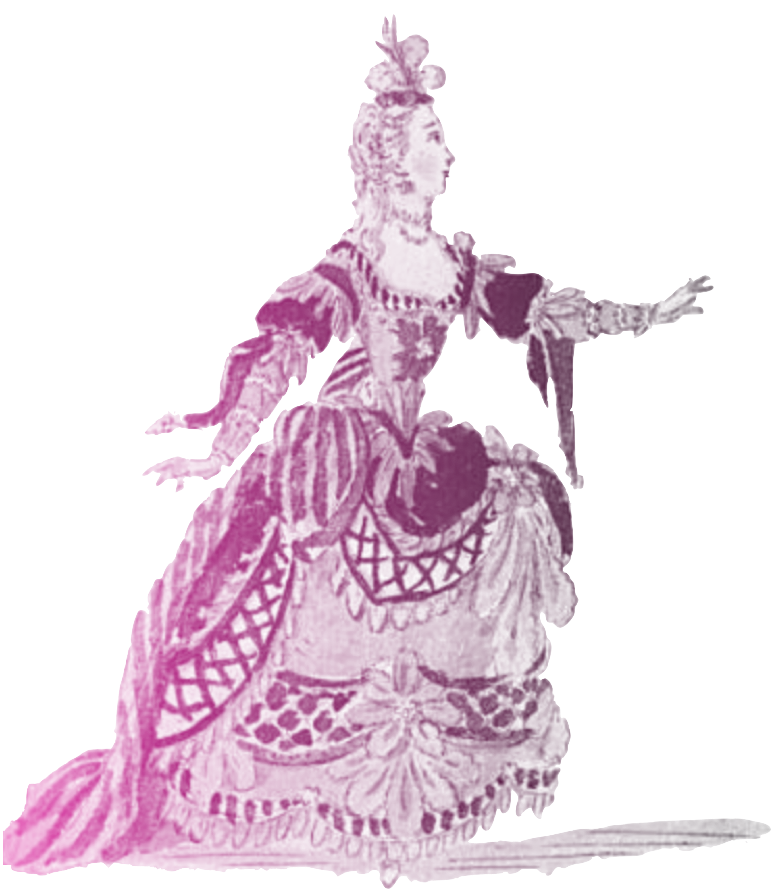
\includegraphics[width=.4\textwidth]{Phani.png}
\end{center}
\vfill




\newpage
\begingroup
\parindent 0pt
\parskip 2ex
\def\enotesize{\normalsize}
\theendnotes
\endgroup

\newpage
\selectlanguage{american}
\addcontentsline{toc}{section}{Works Cited}\secheadr{Works Cited}
\printbibliography

\end{document}